\documentclass[aps,preprint,nofootinbib,floatfix]{revtex4-1}

\usepackage{amsmath,amssymb,amsfonts,amsthm,amscd,bm,bbm}
%\usepackage{nicefrac}       % compact symbols for 1/2, etc.
%\usepackage{microtype}      % microtypography
%\usepackage{mathtools}
%\usepackage{printlen}
%\usepackage{cite}
\usepackage[inline]{enumitem}
\usepackage[inline]{enumitem}
\usepackage[pdftex]{graphicx}
\graphicspath{{./figs/}}
\usepackage{algorithmic}
\usepackage{algorithm}
%\usepackage[none]{hyphenat}
\usepackage{multirow}
\usepackage{colortbl}
\usepackage{array,booktabs}
\usepackage{xcolor}
\usepackage{makecell}

%\pretolerance=10000
%\tolerance=2000 
%\emergencystretch=10pt

\newtheorem{theorem}{Theorem}
\newtheorem{definition}[theorem]{Definition}
\newtheorem{assumption}[theorem]{Assumption}
\newtheorem{lemma}[theorem]{Lemma}
\newtheorem{corollary}[theorem]{Corollary}
\newtheorem{proposition}[theorem]{Proposition}
\newtheorem{conjecture}[theorem]{Conjecture}
\newtheorem{remark}[theorem]{Remark}
\newtheorem{example}{Example}

\DeclareMathOperator{\aff}{aff}
\DeclareMathOperator{\st}{s.t.}
\DeclareMathOperator{\affnot}{aff_0}
\DeclareMathOperator{\conv}{conv}
\DeclareMathOperator{\relint}{relint}
\DeclareMathOperator{\vol}{vol}
\DeclareMathOperator{\range}{range}
\DeclareMathOperator{\image}{im}
\DeclareMathOperator{\nullspace}{null}
\DeclareMathOperator{\area}{area}
\DeclareMathOperator{\vspan}{span}
\DeclareMathOperator{\id}{Id}
\DeclareMathOperator{\cond}{cond}
\DeclareMathOperator{\prox}{prox}
\DeclareMathOperator*{\argmax}{arg\,max}
\DeclareMathOperator*{\argmin}{arg\,min}
\DeclareMathOperator*{\minimize}{minimize}
\DeclareMathOperator{\diag}{diag}
\DeclareMathOperator{\Tr}{Tr}

\newcommand\Energy{\mathcal{E}}
\newcommand\EnergyH{\mathcal{E}^{H}}
\newcommand\EnergyL{\mathcal{E}^{L}}
\newcommand\EnergyOne{\mathcal{E}^{1D}}
\newcommand\E{\mathbb{E}}
\newcommand\kk{K}
\newcommand\kkk{h}
\newcommand\Hk{{\mathcal{H}}_{\kk}}
\newcommand\HH{\mathcal{H}}
\newcommand\C{{\mathcal{C}}}
\newcommand\tC{{\widetilde{\C}}}
\newcommand\OO{{\mathcal{O}}}
\newcommand\Zt{Y}
\newcommand{\Ind}[1]{\mathbbm{1}_{#1}}
\newcommand\e{e}
\newcommand\om{\omega}
\newcolumntype{g}{>{\columncolor{gray!20}}l}


\begin{document}

\title{Energy Clustering}

\author{Guilherme Fran\c ca}
\email{guifranca@gmail.com} 
\author{Joshua T. Vogelstein}
\email{jovo@jhu.edu}
\affiliation{Johns Hopkins University}


\begin{abstract}
Energy statistics was proposed by Sz\' ekely in the 80's inspired by the 
Newtonian gravitational potential from classical mechanics, and it provides 
a non-parametric hypothesis test for equality of distributions. 
It was further generalized from Euclidean spaces to metric spaces of 
strong negative type, and more recently, a connection with reproducing 
kernel Hilbert spaces (RKHS) was established. 
Here we consider the problem of clustering data from an 
energy statistics theory perspective.
We provide a precise mathematical formulation 
yielding a quadratically constrained 
quadratic program (QCQP) in the associated RKHS. We show that this QCQP
is equivalent to kernel $k$-means optimization problem, once the kernel
is fixed.
Thus, our results imply a first principles derivation of kernel $k$-means 
from energy statistics.
However, energy statistics fixes a family of standard kernels.
Furthermore, we also consider a weighted version of energy statistics, 
making connection to graph partitioning problems.
To find local optimizers of such QCQP we consider an iterative algorithm based 
on Hartigan's method, which in this case has the same computational cost 
as kernel $k$-means algorithm, based on Lloyd's method, but usually 
with better clustering quality. 
We provide carefully designed numerical experiments showing the superiority 
of the proposed method compared to kernel $k$-means, standard $k$-means, 
and Gaussian mixture models in a variety of settings.
\end{abstract}

% @gui: you didn't update the abstract?

\maketitle



% @gui: my experience is that most reviewers absolutely do *NOT* want a ToC, rather, we skip it, and journals often remove it prior to publication.


%%%%%%%%%%%%%%%%%%%%%%%%%%%%%%%%%%%%%%%%%%%%%%%%%%%%%%%%%%%%%%%%%%%%%%%%%%%%%%%
\section{Introduction}

Energy statistics \cite{Szkely2013}
is based on a 
notion of statistical potential energy between probability distributions,
in close analogy to Newton's gravitational potential in classical mechanics. 
It provides a non-parametric hypothesis test for equality of 
distributions which is achieved 
under minimum energy. When probability distributions are different the 
statistical potential energy diverges as sample size increases, while tends 
to a nondegenerate limit distribution when probability
distributions are equal. 
Energy statistics has been applied to several goodness-of-fit 
hypothesis tests, multi-sample tests of equality of distributions, 
analysis of variance \cite{RizzoVariance}, nonlinear dependence tests through
distance covariance and distance correlation, which generalizes the Pearson
correlation coefficient, and hierarchical clustering \cite{RizzoClustering} 
by extending Ward's method of minimum variance. Moreover, an application of 
energy statistics to clustering was already proposed \cite{Kgroups}, 
which in part motivated this paper. We refer the reader to \cite{Szkely2013}, 
and references therein, for an overview of energy statistics theory and 
its applications.

In its original formulation, energy statistics has a compact representation
in terms of expectations of pairwise Euclidean distances, providing
straightforward empirical estimates. 
The notion of distance covariance was further generalized from Euclidean 
spaces to metric spaces of strong negative type \cite{Lyons}. Furthermore, 
the missing link between energy distance based tests and kernel 
based tests has 
been recently resolved \cite{Sejdinovic2013}, where a unifying framework
establishing an equivalence between generalized energy distances to maximum
mean discrepancies (MMD), which are distances between embeddings of 
distributions in reproducing kernel Hilbert spaces (RKHS), was established. 
This equivalence immediately relates energy statistics to
kernel methods, often used in machine learning, and form the basis 
of our approach.

Clustering has such a long history in machine learning, making it
impossible to mention all important contributions in a short space. 
Perhaps, the most used method is $k$-means \cite{Lloyd,MacQueen,Forgy}, which
is based on Lloyd's heuristic \cite{Lloyd} of assigning a data point to
the cluster with closest center. The only statistical 
information about each cluster comes from its mean, making it sensitive 
to outliers. Nevertheless, $k$-means works very well when data is 
linearly separable in Euclidean space. Gaussian mixture models (GMM) is 
another very common approach, providing more flexibility than $k$-means, 
however, it still makes strong assumptions about the distribution of 
the data.

To account for nonlinearities, kernel methods were introduced 
\cite{Smola,Girolami}. A mercer kernel \cite{Mercer} is used to implicitly
map data points to a RKHS, then clustering can be performed in the associated
Hilbert space by using its inner product. However, the kernel choice remains 
the biggest challenge since there is no principled theory to construct a kernel
for a given dataset, and usually a kernel introduces hyperparameters that 
need to be carefully chosen.
The well-known kernel $k$-means optimization problem is nothing but $k$-means 
in the feature space \cite{Girolami}. Furthermore, kernel $k$-means algorithm
\cite{Dhillon2,Dhillon} is still based on Loyd's heuristic \cite{Lloyd}
of grouping points that are closer to a cluster center, now
in feature space. 
We refer the reader to \cite{Filippone} for a survey of clustering
methods.

Although clustering from energy statistics was considered
in \cite{Kgroups}, the precise optimization problem behind this approach
remains elusive, as well as the connection with kernel methods.
The main theoretical contribution of this paper is to fill this gap.
Since the statistical potential energy is minimum when
distributions are equal, the principle behind clustering is to maximize 
the statistical energy,  enforcing probability distributions associated to 
each cluster to be different from one another. We provide a precise 
mathematical formulation to this statement, leading to a quadratically 
constrained quadratic program (QCQP) in the associated RKHS. Our results
immediately establish the connection with kernel methods, showing that this 
QCQP is equivalent to kernel $k$-means optimization problem. The 
equivalence between kernel $k$-means, spectral clustering, and graph 
partitioning problems is well-known \cite{Dhillon,Dhillon2}. We demonstrate 
how these relations arise from a weighted version of energy statistics.

Our main 
algorithmic contribution is to use Hartigan's method \cite{Hartigan} to 
find local solutions of the above mentioned QCQP, which is NP-hard in general.
Hartigan's method was also used in \cite{Kgroups}. More importantly, its 
advantages
over Lloyd's method was already demonstrated 
in some simple settings
\cite{Telgarsky,Slonin}, but apparently this method did not receive 
the deserved attention. To the 
best of our knowledge, Hartigan's method was not previously 
employed together with kernel methods. 
We provide a full kernel based Hartigan's algorithm for clustering,
where the kernel is fixed by energy statistics. 
We make clear the advantages of this proposal versus 
Lloyd's method, which kernel $k$-means is based upon and will also be used 
to solve our QCQP. We show that both algorithms  have the same
time complexity, but Hartigan's method in kernel spaces offer several
advantages. Furthermore, in the examples considered in this paper, it 
also provides superior performance compared to a spectral clustering
relaxation of the QCQP.

Our numerical results provide compelling evidence that 
Hartigan's method applied to energy statistics based clustering, 
or \emph{energy clustering} for short, is more accurate and robust than 
Lloyd's method. Our experiments also put in evidence the
flexibility of energy clustering, which provides a family of default kernels, 
showing that it is able to perform accurately on data coming from 
very different distributions, contrary to $k$-means and GMM for instance.
More specifically, our algorithms for energy clustering perform 
closely to $k$-means and GMM on normally distributed data, but on the other
hand, performs considerably better than $k$-means and GMM on  data that 
is not normally distributed. It also performs better than $k$-means 
and GMM in high dimensions, even on Gaussian settings. However, it performs 
worse than GMM, and more closely to $k$-means, for highly unbalanced clusters
with normal distributions.

Our work is organized as follows. In section~\ref{sec:background}, we introduce
the necessary background on energy statistics and RKHS.
Section~\ref{sec:clustering_theory} contains the main theoretical 
results of this paper,
where we consider a clustering theory based on energy statistics leading
to a QCQP, which is NP-hard in general. We also show the equivalence to 
kernel $k$-means optimization problem.
In Section~\ref{sec:weighted}, we generalize these results to a weighted
version of energy statistics, providing connections to graph
partitioning problems.
In Section~\ref{sec:twoclass}, we consider the  simple case of a two-class
problem in one dimension,
where we propose an algorithm which requires no random initialization.
In section~\ref{sec:algo}, we consider Lloyd's and Hartigan's methods
and propose iterative algorithms to solve the QCQP.
Section~\ref{sec:numerics} contains some carefully designed numerical
experiments showing that, in a variety of settings, energy clustering based
on Hartigan's algorithm
outperform $k$-means, GMM, kernel $k$-means, and a version of
spectral clustering.
Our final conclusions are presented in Section~\ref{sec:conclusion}.


%%%%%%%%%%%%%%%%%%%%%%%%%%%%%%%%%%%%%%%%%%%%%%%%%%%%%%%%%%%%%%%%%%%%%%%%%%%%%%%
\section{Background on Energy Statistics and RKHS}
\label{sec:background}

% @gui: i'm not sure the above is true/meaningful.  nonparametric means implicitly estimating an infinite number of parameters.  without any statistical theory, i'm not quite sure what we can say.
% @jovo: I stopped saying non-parametric, however, Kolmogorov-Smirnov is also
% said to be non-parametric. I think non-parametric tests also mean that
% it does not assume any form of distributions, i.e. it is a distribution-free
% statistical test.
% @gui: KS test is nonparametric because it can reject for any distribution, we cannot cluster for any distribution, so we are not.


In this section we introduce the main concepts from energy
statistics and its relation to 
RKHS which form the basis of our work.
For more details we refer the reader
to \cite{Szkely2013} and \cite{Sejdinovic2013}.

Consider random variables in $\mathbb{R}^D$ 
such that $X,X' \stackrel{iid}{\sim} P$ and 
$Y,Y' \stackrel{iid}{\sim} Q$, where $P$ and $Q$ are cumulative
distribution functions with finite first moments. 
The quantity 
\begin{equation}
\label{eq:energy}
\Energy(P, Q) \equiv 2 \E \| X - Y\| - \E \| X - X' \| - \E \| Y - Y' \|,
\end{equation}
called \emph{energy distance} \cite{Szkely2013}, 
is rotationally invariant and nonnegative, $\Energy(P,Q) \ge 0$, where
equality
to zero holds if and only if $P = Q$.
Above, $\| \cdot \|$ denotes the
Euclidean norm in $\mathbb{R}^D$. 
Energy distance
provides a characterization of equality of distributions, and
$\Energy^{1/2}$ is
a metric on the space of distributions.

The energy distance can be generalized as, for instance,
\begin{equation}
\label{eq:energy2}
\Energy_\alpha(P, Q) \equiv 
2 \E \| X - Y\|^{\alpha} - \E \| X - X' \|^{\alpha} - 
\E \| Y - Y' \|^{\alpha}
\end{equation}
where $0<\alpha\le 2$. This quantity is also nonnegative,
$\Energy_\alpha(P,Q) \ge 0$. Furthermore, for $0<\alpha<2$ we have that
$\Energy_\alpha(P,Q) = 0$ if and only if $P=Q$, while for $\alpha=2$ 
we have $\Energy_2(P,Q) = 2\| \E(X) - \E(Y) \|^2$ which shows that
equality to zero only requires
equality of the means, and thus $\Energy_2(P,Q)=0$ does 
not imply equality of distributions.

The energy distance can be even further generalized.
Let $X, Y \in \mathcal{X}$  where $\mathcal{X}$ is an arbitrary space endowed
with a \emph{semimetric of negative type}
$\rho: \mathcal{X}\times\mathcal{X} \to \mathbb{R}$, which is required
to satisfy
\begin{equation}
\label{eq:negative_type}
\sum_{i,j=1}^n c_i c_j \rho(X_i, X_j) \le 0,
\end{equation}
where $X_i \in \mathcal{X}$ and $c_i \in \mathbb{R}$ such that
$\sum_{i=1}^n c_i = 0$. Then, $\mathcal{X}$ is called a \emph{space of
negative type}.
We can thus replace $\mathbb{R}^D \to \mathcal{X}$ and 
$\| X - Y \| \to \rho(X , Y)$ in the definition \eqref{eq:energy}, obtaining
the generalized energy distance
\begin{equation}
\label{eq:energy3}
\Energy(P, Q) \equiv 2 \E \rho(X,Y) - \E \rho(X, X') - \E \rho(Y,Y').
\end{equation}
For spaces of negative type there exists a Hilbert space $\mathcal{H}$ and
a map $\varphi: \mathcal{X} \to
\mathcal{H}$ such that
$\rho(X, Y) = \| \varphi(X) - \varphi(Y) \|_{\mathcal{H}}^2$. This
allows us to compute quantities related to probability distributions over
$\mathcal{X}$ in the associated Hilbert space $\mathcal{H}$.
Even though the semimetric 
$\rho$ may not satisfy the triangle inequality, 
$\rho^{1/2}$ does since it can be shown to be a proper metric. 

There is an equivalence between energy distance, 
commonly used in statistics,
and distances between embeddings of distributions in 
RKHS, commonly used in machine learning. 
This equivalence was established
in \cite{Sejdinovic2013}. Let us first recall the definition of
RKHS. Let $\HH$ be a Hilbert space of real-valued functions
over $\mathcal{X}$. A function 
$\kk : \mathcal{X} \times \mathcal{X} \to 
\mathbb{R}$ is a reproducing kernel of $\HH$ if it satisfies
the following two conditions:
\begin{enumerate}
\item $\kkk_x \equiv \kk(\cdot, x) \in \HH$ 
for all $x \in \mathcal{X}$.
\item $\langle \kkk_x, f \rangle_{\HH} = f(x)$ for
all $x\in\mathcal{X}$ and $f\in \HH$.
\end{enumerate}
In other words, for any $x \in \mathcal{X}$ and any function $f \in \HH$,
there is a unique 
$\kkk_x \in \HH$ that reproduces $f(x)$ through the inner product
of $\HH$.
If such a \emph{kernel} 
function $\kk$ exists, then $\HH$ is called a RKHS. The above two 
properties immediately imply that $\kk$ is symmetric and positive
definite. Indeed, notice that
$\langle \kkk_x, \kkk_y \rangle = \kkk_y(x) = \kk(x,y)$, and by 
definition 
$\langle \kkk_x, \kkk_y \rangle^* = \langle \kkk_y, \kkk_x \rangle$, but
since the inner product is real we have 
$\langle \kkk_y, \kkk_x \rangle = \langle \kkk_x, \kkk_y \rangle$, or
equivalently 
$\kk(y,x) = \kk(x,y)$. Moreover, for any $w \in
\HH$ we can write $w = \sum_{i=1}^n c_i \kkk_{x_i}$ where
$\{ \kkk_{x_i} \}_{i=1}^n$ is a basis of $\HH$. It follows that
$\langle w, w \rangle_{\HH}  = \sum_{i,j=1}^n c_i c_j \kk(x_i,x_j) \ge 0$,
showing that the kernel is positive definite. If $G$ is a matrix with
elements $G_{ij} = \kk(x_i,x_j)$ this is equivalent to $G$ being
positive semidefinite, i.e. $v^\top G \, v \ge 0$ for any vector
$v \in \mathbb{R}^n$.

The Moore-Aronszajn theorem 
\cite{Aronszajn}
establishes the converse of the above paragraph. 
For every symmetric
and positive definite function $\kk: \mathcal{X}\times \mathcal{X} \to
\mathbb{R}$, there is an associated RKHS $\Hk$ 
with reproducing
kernel $\kk$. The map $\varphi: x \mapsto \kkk_x \in \Hk$ is called
the canonical \emph{feature map}. Given a kernel $\kk$,
this theorem enables us to define an embedding of a probability measure
$P$ into the RKHS as follows: $P \mapsto \kkk_P \in
\Hk$ such that 
$\int f(x) d P(x) = \langle f, \kkk_P \rangle$ for all $f \in \Hk$,
or alternatively, $\kkk_P \equiv \int \kk( \, \cdot \,, x)  d P(x)$. 
We can now  introduce the 
notion of distance between two probability measures using the inner product
of $\Hk$, which is called the maximum mean discrepancy (MMD) and
is given by
\begin{equation}
\label{eq:mmd}
\gamma_\kk(P,Q) \equiv \| \kkk_P - \kkk_Q \|_{\Hk}.
\end{equation}
This can also be written as \cite{Gretton2012}
\begin{equation}\label{eq:mmd2}
\gamma_\kk^2(P,Q) = \E \kk(X,X') + \E \kk(Y,Y') - 2 \E \kk(X, Y)
\end{equation}
where $X,X' \stackrel{iid}{\sim} P$ and $Y,Y'\stackrel{iid}{\sim} Q$.
From the equality between \eqref{eq:mmd} and \eqref{eq:mmd2} we also
have 
\begin{equation}\label{eq:inner_data}
\langle \kkk_P, \kkk_Q \rangle_{\Hk} = \E \, \kk(X, Y).
\end{equation}
Thus, in practice, we can estimate the inner product between  
embedded distributions 
by averaging the kernel function over sampled data.

The following important result shows that semimetrics of negative
type and symmetric positive definite kernels are closely related
\cite{Berg1984}. Let $\rho: \mathcal{X} \times \mathcal{X} \to \mathbb{R}$
and $x_0 \in \mathcal{X}$ an arbitrary but fixed point.
Define
\begin{equation}
\label{eq:kernel_semimetric}
\kk(x,y) \equiv 
\tfrac{1}{2} \left[  \rho(x,x_0) + \rho(y,x_0) - \rho(x,y)\right].
\end{equation}
Then, it can be shown that 
$\kk$ is positive definite if and only if $\rho$ is a semimetric
of negative type.
We have a family of kernels, one for each choice of $x_0$. Conversely,
if $\rho$ is a semimetric of negative type and $\kk$ is a kernel in this
family, then 
\begin{equation}
\label{eq:gen_kernel}
\begin{split}
\rho(x,y) &= \kk(x,x) + \kk(y,y) -2\kk(x,y) \\
&=  \| \kkk_x - \kkk_y \|^2_{\Hk}
\end{split}
\end{equation}
and the canonical feature map 
$\varphi: x \mapsto \kkk_x$ is injective \cite{Sejdinovic2013}.
When these conditions are satisfied we say that the kernel $\kk$ 
generates the semimetric $\rho$. 
If two different kernels generate the same $\rho$ they are
said to be equivalent kernels.

Now we can state the equivalence between energy distance $\Energy$ and
inner products on RKHS, which is one of the main results of
\cite{Sejdinovic2013}. If $\rho$ is a semimetric
of negative type and $\kk$ a kernel that generates $\rho$, then
replacing \eqref{eq:gen_kernel} into
\eqref{eq:energy3}, and using \eqref{eq:mmd2}, yields
\begin{equation} \label{eq:Erho}
\Energy(P, Q) = 
2 \left[ \E \, \kk(X, X') + \E \, \kk(Y, Y') - 2\E \, \kk(X, Y)\right] 
= 2 \gamma_\kk^2(P,Q) .
\end{equation}
Due to \eqref{eq:mmd} we can compute the energy 
distance $\mathcal{E}(P, Q)$ between two probability distributions
using the inner 
product of $\Hk$. 

Finally, let us recall the main formulas from energy statistics
for the test statistic of equality of distributions \cite{Szkely2013}. 
Assume we have data $\mathbb{X} = \{ x_1,\dotsc, x_n \}$ where
$x_i \in \mathcal{X}$, and $\mathcal{X}$ is a space of negative type.
Consider a disjoint partition $\mathbb{X} = \bigcup_{j=1}^k \C_j$, with
$\C_i \cap \C_j = \emptyset$.
Each expectation in the generalized energy distance
\eqref{eq:energy3}
can be computed 
through the function
\begin{equation}
\label{eq:g_def}
g (\C_i, \C_j) \equiv 
\dfrac{1}{n_i n_j}
\sum_{x \in \C_i} 
\sum_{y \in \C_j} \rho(x, y) ,
\end{equation}
where $n_i = |\C_i|$ is the number of elements in partition
$\C_i$. 
The \emph{within energy dispersion} is defined by
\begin{equation}
\label{eq:within}
W \equiv
\sum_{j=1}^{k} \dfrac{n_j}{2} g(\C_j, \C_j),
\end{equation}
and the \emph{between-sample energy statistic} is defined by
\begin{equation}
\label{eq:between}
S \equiv
\sum_{1 \le  i < j \le k } \dfrac{n_i n_{j}}{2 n} \left[
2 g(\C_i, \C_j) - 
g(\C_i, \C_i) - 
g(\C_j, \C_j)
\right],
\end{equation}
where $n = \sum_{j=1}^k n_j$.
Given a set of distributions
$\{ P_j\}_{j=1}^k$, where $x \in \C_j$ if and only if $x \sim P_j$, 
the quantity $S$ provides
a test statistic for equality of distributions
\cite{Szkely2013}.
When the sample size is large enough, $n\to \infty$,
under the null hypothesis $H_0: P_1=P_2=\dotsm=P_k$ we have that
$S\to 0$, 
and under
the alternative hypothesis $H_1: P_i \ne P_j$ for at least two $i\ne j$, 
we have that $S \to \infty$.
Note that this test does not make any assumptions
about the distributions $P_j$, thus it is said to be non-parametric or
distribution-free.

One can make a physical analogy by thinking 
that points $ x \in \C_j$ form a massive body 
whose total mass is characterized by the distribution function $P_j$.
The quantity $S$ is thus a potential
energy of the from $S(P_1,\dotsc,P_k)$ which measures how different
the distribution of these masses are,  and achieves the ground state
$S=0$ when all bodies have the same mass distribution. The potential energy
$S$ increases as bodies have different mass distributions.


%%%%%%%%%%%%%%%%%%%%%%%%%%%%%%%%%%%%%%%%%%%%%%%%%%%%%%%%%%%%%%%%%%%%%%%%%%%%%%%
\section{Clustering Based on Energy Statistics}
\label{sec:clustering_theory}

% @gui: consider only using equation numbers for equations that you later refer to? there are so many, it is easy to get lost.
% @jovo: ok, will do that after we finish everything. There is a package that
% automatically remove numbers from unreferenced equations. It is a common
% practice however to number every equation in the paper,
% specially for reviewing purposes. But later 
% I will remove the numbers from the not cited ones if you don't like
% @gui: maybe common in math, but certainly not in stats / data science. 
% in any case, what is the package that does that?


% @gui: do other people know this result? (about min W = max X) if so, cite them, if not, state that.
% @jovo: eq (15), i.e. S + W = T is well-known. Gabor and Rizzo wrote that
% in their paper, however, they didn't write a proof. They should have
% it in some other paper.  However, they mention 
% that this holds only for 0 < alpha < 2, with |x-y|^alpha, while
% here I did for a general semimetric. Thus I don't really know if in general
% this is equality is known or not, but it should because it's a very easy
% derivation. The PhD thesis do not 
% mention anywhere that minimizing W is equivalent to maximizing S.
% Therefore, I don't want to sound like this is a big result and possibly
% a referee can say  "well this is trivial and known".
% Thus I just preferred to do my own derivation and not say anything.
% What do you think??
% @gui: i'd state it as a lemma then.




% @gui: i'm not sure about this.  who is to say the correct direction of causality? maybe energy clustering is a special case of kernel k-means?
% @jovo: I tried to not commit to a single view. We show they are
% equivalent, when opperating on the same kernel. However, kernel k-means per
% se does not consider anything about the kernel choice. Energy statistics,
% however, provides a theory valid on spaces of negative type, which guarantees
% that a kernel constructed within this formalism will be 
% positive-semidefinite. Thus, I still prefer to look in the first direction.
% @gui: ok, did you update the text? i don't recall where i made this comment and don't want to search for it again. can you point me to the place that you say this?

This section contains the main theoretical results of this paper, where 
we formulate an optimization problem for clustering 
based on energy statistics and RKHS introduced in the previous section.

Due to the energy test statistic for equality of distributions,
the obvious
criterion for clustering data is to 
maximize $S$ which makes 
each cluster as different
as possible from the other ones.
In other words, given a set of points coming from different probability
distributions, the test statistic $S$ should attain a maximum when 
each point is correctly
classified as belonging to the cluster associated to its probability
distribution.
The following 
straightforward result
shows that maximizing $S$ is, however, equivalent to minimizing
$W$ which has a more convenient form.

\begin{proposition}
\label{th:minimize}
Let $\mathbb{X} = \{x_1,\dotsc,x_n\}$ where each data point
$x_i$ lives in a space $\mathcal{X}$ endowed with a semimetric $\rho:
\mathcal{X}\times\mathcal{X} \to \mathbb{R}$ of
negative type. For a fixed integer $k$,
the partition
$\mathbb{X} = \bigcup_{j=1}^k \C_j$, where $\C_i \cap C_j = \emptyset$ for
all $i\ne j$, maximizes the between-sample statistic $S$, defined
in equation \eqref{eq:between}, if and only if
\begin{equation}
\label{eq:minimize}
\min_{\C_1,\dotsc,C_k  } W(
\C_1, \dotsc, \C_k),
\end{equation}
where the within energy dispersion $W$ is defined by \eqref{eq:within}.
\end{proposition}
\begin{proof}
From \eqref{eq:within} and \eqref{eq:between}
we have
\begin{equation}
\begin{split}
S + W &= 
\dfrac{1}{2n} \sum_{\substack{i,j=1 \\ i\ne j}}^k n_i n_j g(\C_i, \C_j)
+ \dfrac{1}{2n} \sum_{i=1}^{k} 
\bigg[ n - 
\sum_{j\ne i = 1}^k n_j \bigg] 
n_i g(\C_i, \C_i) \\
& = \dfrac{1}{2n} \sum_{i,j=1}^k n_i n_j g(\C_i, \C_j)
= \dfrac{1}{2n} \sum_{x \in \mathbb{X}} \sum_{y \in \mathbb{X}} \rho(x,y)
= \dfrac{n}{2} g(\mathbb{X}, \mathbb{X}).
\end{split}
\end{equation}
Note that the right hand side of this equation 
only depends on the pooled data, so it is a constant
independent of the choice of partition. Therefore, maximizing
$S$ over the choice of partition is equivalent to minimizing $W$.
\end{proof}

For a given $k$, the clustering problem amounts to
finding the best partition of the data by minimizing $W$.
Notice that this is a hard clustering problem as partitions
are disjoint. The optimization problem \eqref{eq:minimize} based on
energy statistics was already proposed in \cite{Kgroups}. However, it is
important to note that this is equivalent to maximizing $S$,
which is the test statistic for equality of distributions. In this current
form, the relation with kernels and other clustering methods is obscure.
In the following, we show what is the explicit optimization problem behind 
\eqref{eq:minimize} in the corresponding RKHS, 
establishing the connection with kernel methods.

Based on the relation between kernels and semimetrics of negative
type, 
assume that the kernel $\kk: \mathcal{X} \times \mathcal{X} \to \mathbb{R}$ 
generates $\rho$.  Define  the Gram matrix
\begin{equation}
\label{eq:kernel_matrix}
G \equiv \begin{pmatrix}
\kk(x_1,x_1) & \kk(x_1,x_2) & \dotsm & \kk(x_1,x_n) \\
\kk(x_2,x_1) & \kk(x_2,x_2) & \dotsm & \kk(x_2,x_n) \\
\vdots & \vdots & \ddots  & \vdots \\
\kk(x_n,x_1) & \kk(x_n,x_2) & \dotsm & \kk(x_n,x_n) 
\end{pmatrix} .
\end{equation}
Let $Z \in \{ 0,1 \}^{n\times k}$ be the label matrix, 
with only one nonvanishing entry per row, 
indicating to which cluster (column)
each point (row) belongs to. This matrix satisfies
$Z^\top Z = D$, where the diagonal matrix 
$D = \diag( n_1,\dotsc, n_k )$  contains
the number of points in each cluster. We also introduce the rescaled
matrix  $Y \equiv Z D^{-1/2}$. In component form they are given by
\begin{equation}
\label{eq:label_matrix}
Z_{ij} \equiv \begin{cases}
1 & \mbox{if $x_i \in \C_j$ } \\
0 & \mbox{otherwise}
\end{cases} \qquad
\Zt_{ij} \equiv \begin{cases}
\tfrac{1}{\sqrt{n_j}} & \mbox{if $x_i \in \C_j$ } \\
0 & \mbox{otherwise}
\end{cases} .
\end{equation}
Throughout the paper, we use the notation $M_{i\bullet}$ to denote
the $i$th row of a matrix $M$, and $M_{\bullet j}$ denotes its $j$th column.
Our next result shows that the optimization problem \eqref{eq:minimize}
is NP-hard since
it is a quadratically constrained quadratic program (QCQP) in the RKHS.

\begin{proposition} 
\label{th:qcqp2}
The optimization problem \eqref{eq:minimize} is equivalent to
\begin{equation}
\label{eq:qcqp2}
\max_{\Zt} \Tr \left( \Zt^\top G \, \Zt \right)  \qquad
\mbox{s.t. $\Zt \ge 0$, $\Zt^\top \Zt = I$, 
$\Zt \Zt^\top \e = \e$},
\end{equation}
where $\e = (1,1,\dots,1)^\top \in \mathbb{R}^n$ is the all-ones vector,
and $G$ is the Gram matrix \eqref{eq:kernel_matrix}.
\end{proposition}
\begin{proof}
From 
\eqref{eq:gen_kernel},
\eqref{eq:g_def}, and
\eqref{eq:within}
we have
\begin{equation}
\label{eq:W2}
W(\C_1,\dotsc,\C_k  )
= \dfrac{1}{2} \sum_{j=1}^k \dfrac{1}{n_j} \sum_{x,y \in \C_j} \rho(x,y)
= \sum_{j=1}^k \sum_{x \in \C_j}  \bigg(
\kk(x,x) - \dfrac{1}{n_j} \sum_{y \in \C_j} \kk(x,y) \bigg).
\end{equation}
Note that the first term is global so it does not contribute to the 
optimization problem.
Therefore, minimizing \eqref{eq:W2} is equivalent to
\begin{equation}
\label{eq:max_prob}
\max_{ \C_1,\dotsc,\C_k } 
\sum_{j=1}^k \dfrac{1}{n_j} \sum_{x,y\in C_j} \kk(x,y) .
\end{equation}
But 
\begin{equation}
\sum_{x, y \in \C_j} \kk(x, y) =
\sum_{p=1}^{n} \sum_{q=1}^{n} Z_{pj} Z_{qj} G_{pq} = 
(Z^\top G \, Z)_{jj},
\end{equation}
where we used the definitions \eqref{eq:kernel_matrix} and
\eqref{eq:label_matrix}. Thus, the objective function in 
\eqref{eq:max_prob} is equal to
$\Tr \left( D^{-1} Z^\top G Z \right)$. 
% @gui: the above step is not obvious
% @jovo: It is obvious. 
% From (21) we have \sum_j 1/n_j (Z^T G Z)_jj. But 1/n_j is just
% D^{-1}_jj (the diagonal matrix). The sum over j goes over the diagonals of
% D^{-1} Z^T G Z which is the definition of the trace
% @gui: obvious to you \neq obvious.  i understood, i want you to explain it.
Now we can
use the cyclic property
of the trace, and by the  definition of the matrix $Z$
in \eqref{eq:label_matrix}, we obtain the following integer
programing problem:
\begin{equation}\label{eq:qcqp}
\max_{Z} \Tr\Big( \big( Z D^{-1/2}\big)^\top G 
\big( ZD^{-1/2} \big) 
\Big) \quad
\mbox{s.t. $Z_{ij} \in \{0,1\}$, $\sum_{j=1}^k Z_{ij} = 1$, 
$\sum_{i=1}^n Z_{ij} = n_j$.}
\end{equation}

Now we write this in terms of the matrix $Y = Z D^{-1/2}$.
The objective function immediately becomes
$\Tr\left( Y^\top G \, Y\right)$. Notice that the above constraints
imply that $Z^T Z = D$, where $D=\diag(n_1,\dotsc,n_k)$, which in turn gives
$D^{-1/2} Y^T Y D^{-1/2} = D$, or $Y^\top Y = I$. 
Also, every entry of $Y$ is positive by definition,
$Y \ge 0$. Now it only remains to show the last 
constraint in \eqref{eq:qcqp2}, which comes from the last
constraint in \eqref{eq:qcqp}. In matrix form this reads
$Z^T \e = D \e$. Replacing $Z=YD^{1/2}$ we have
$Y^\top \e = D^{1/2} \e$. Multiplying this last equation
on the left by $Y$, and noticing
that $Y D^{1/2} \e = Z \e = \e$, we finally obtain
$Y Y^\top \e = \e$. Therefore, the optimization 
problem \eqref{eq:qcqp} is equivalent
to \eqref{eq:qcqp2} .
\end{proof}

Based on Proposition~\ref{th:qcqp2}, to group data
$\mathbb{X} = \{ x_1,\dotsc,x_n \}$
into  $k$ clusters we first compute the Gram matrix
$G$ and then 
solve the optimization problem \eqref{eq:qcqp2} for $\Zt \in
\mathbb{R}^{n\times k}$. The $i$th row
of $\Zt$ will contain a single nonzero element in some $j$th column,
indicating that $x_i \in \C_j$. 
This optimization problem is nonconvex, and also NP-hard,
thus a direct approach 
is computational prohibitive even for small datasets.
However, one can find approximate solutions by relaxing some 
of the constraints, or obtaining a relaxed SDP version of it.
For instance, the relaxed problem
\begin{equation}
\label{eq:relaxed}
\max_{Y} \Tr \left( Y^\top G \, Y \right) \quad \mbox{s.t. $Y^\top Y = I$}
\end{equation}
has a well-known closed form solution $Y^\star = U R$, where the
columns of $U \in \mathbb{R}^{n\times k}$ 
contain the top $k$ eigenvectors of $G$ corresponding
to the $k$ largest eigenvalues $\lambda_1\ge \lambda_2\ge\dotsc\ge\lambda_k$, 
and
$R \in \mathbb{R}^{k\times k}$ is an arbitrary orthogonal matrix. 
The resulting
optimal objective function assumes the value 
$\max \Tr \left( {Y^\star}^\top G \, Y^\star \right)  = 
\sum_{i=1}^k \lambda_i$. 

Spectral clustering is based on the above approach, where
one further normalize the rows of $Y^\star$, 
i.e. $Y^\star \to \widetilde{Y}$ where 
$\widetilde{Y}_{ij} \equiv Y^\star_{ij} \big/ \| Y^\star_{i\bullet} \|$. 
The vectors
$y_i \equiv \widetilde{Y}_{i\bullet} \in \mathbb{R}^k$, which are the
rows of matrix $\widetilde{Y}$, lie on the surface of the $k$-dimensional 
unit sphere.
The set $\{ y_i \}_{i=1}^n$ is a spectral embedding of the original
set $\{ x_i \}_{i=1}^n$ onto an eigen-subspace of the kernel matrix $G$.
After performing this embedding, one group the points 
$\{ y_i \}_{i=1}^n$ into $k$ clusters 
$\{ \tC_1,\dotsc,\tC_k \}$ using any clustering algorithm, such as
$k$-means. This yields the final solution
where the original point $x_i$ belongs
to cluster $\C_j$ if and only if $y_i$ belongs to $\tC_j$.
A procedure on these lines was proposed in the seminal paper
\cite{NgJordan}, which considers the eigen-decomposition of
the matrix $D^{-1/2} G D^{-1/2}$ instead of $G$, and also 
where $G$ is an affinity matrix with the modification that
its diagonal elements are set to zero $G_{ii}=0$, 
and $D=\diag(d_{1},\dotsc,d_{n})$ is the degree matrix, 
with $d_{i} \equiv \sum_{j=1}^n G_{ij}$. 
We consider a slightly modification of this procedure,
which we call \mbox{$\mathcal{E}^{S}$-clustering} 
to emphasize that its a spectral
method whose kernel comes from energy statistics, by 
computing the 
eigen-decomposition of $G D^{-1}$ instead.
This  method is described in 
Algorithm~\ref{spectralalgo} and will be used as a comparison
to the other iterative algorithms 
that will be proposed later.

\begin{figure}
\begin{flushleft}
\begin{algorithm}[H]
\vspace{.5em}
\begin{algorithmic}[1]
\INPUT Gram matrix $G\in\mathbb{R}^{n\times n}$, and number of clusters $k$
\OUTPUT label matrix $Z \in \{ 0, 1\}^{n \times k}$
\STATE set the diagonal of $G$ to zero: $G_{ii} \leftarrow 0$ 
        for $i=1,\dotsc,n$
\STATE $D\leftarrow\diag(d_1,\dotsc,d_n)$ 
        where $d_i \leftarrow \sum_{j=1}^n G_{ij}$
\STATE solve the generalized eigenvalue problem $G v_i = \lambda_i D v_i$,
        where $i=1,\dotsc,n$ with eigenvalues, and corresponding eigenvectors,
        obeying the ordering
        $\lambda_1 \ge \lambda_2 \ge \dotsc \lambda_n$
\STATE $Y \leftarrow (D v_1| \dotsm | D v_k) 
        \in \mathbb{R}^{n\times k}$ 
has the top $k$ eigenvectors (multiplied by $D$) as columns
\STATE normalize the rows $Y$, i.e. 
$\widetilde{Y}_{ij} \leftarrow Y_{ij} \Big/ 
\left(\sum_{j=1}^n |Y_{ij}|^2\right)^{1/2}$
\STATE apply $k$-means on $\{ y_i \}_{i=1}^n$, 
where $y_i = \widetilde{Y}_{i\bullet}$
is the $i$th row of $\widetilde{Y}$
\STATE $Z_{ij} \leftarrow 1$ if $y_i$ is in cluster $j$, 
        and $Z_{ij} \leftarrow 0$ otherwise
\end{algorithmic}
\caption{
\label{spectralalgo}
$\mathcal{E^S}$-clustering is an exact spectral method to solve
the relaxed problem \eqref{eq:relaxed}.
\hspace{\fill}
}
\end{algorithm}
\end{flushleft}
\end{figure}

Note that the energy clustering problem \eqref{eq:qcqp2} 
is valid for data living in an \emph{arbitrary} space of negative type, where
a semimetric $\rho$, and thus the kernel $\kk$, are
assumed to be known. Standard energy statistics in
Euclidean space fixes a family of choices 
$\rho_\alpha(x,y) = \| x - y\|^\alpha$, with the corresponding
kernel $K_\alpha(x,y) = \tfrac{1}{2} \left( \| x \|^\alpha + \| y \|^\alpha - 
\| x-y\|^\alpha \right)$, where we
set $x_0=0$ in \eqref{eq:kernel_semimetric} and  $0<\alpha\le 2$.
The same would be valid for data living in a more general
metric space $(\mathcal{X}, \rho)$, where the corresponding semimetric $\rho$ 
fixes the kernel.
In any case, the energy  clustering 
formulation does not make assumptions
about  the distribution of the data, 
contrary to $k$-means and GMM, for example.
In practice, however,
the clustering quality strongly depend on the choice of a suitable
$\rho$, which measures the similarity between data points,
and is equivalent to choosing an appropriate kernel.
However, if prior information is available to choose an appropriate $\rho$,
it can be conveniently incorporated in the 
optimization problem \eqref{eq:qcqp2}.


\subsection*{Relation to Kernel $\bm{k}$-Means}

One may wonder how energy clustering 
relates to the well-known kernel $k$-means problem%
\footnote{When we refer to kernel $k$-means problem we mean specifically 
the optimization problem \eqref{eq:kernel_kmeans}, which should not be 
confused with kernel $k$-means algorithm that is just one possible recipe 
to solve \eqref{eq:kernel_kmeans}.} 
which is extensively used in machine learning.
For a positive semidefinite Gram matrix $G$, as defined in
\eqref{eq:kernel_matrix},
there exists a map
$\varphi: \mathcal{X} \to \HH_\kk$ such that
$\kk(x,y) = \varphi(x)^\top \varphi(y)$. The kernel $k$-means optimization
problem,
in feature space,
is defined by
\begin{equation}
\label{eq:kernel_kmeans}
\min_{\C_1,\dotsc,\C_k}\bigg\{ 
J(\C_1,\dots,\C_k) \equiv  \sum_{j=1}^k
\sum_{x \in \C_j} \| \varphi(x) - \varphi(\mu_j) \|^2
\bigg\}
\end{equation}
where $\mu_j = \tfrac{1}{n_j} \sum_{x \in \C_j} x$ is the  mean of cluster
$\C_j$ in the ambient space. Notice that the above objective function
is strongly tied to the idea of minimizing distances between points
and cluster centers, which arises from $k$-means objective function based
on Lloyd's method \cite{Lloyd}.
It is known \cite{Dhillon2,Dhillon}
that problem \eqref{eq:kernel_kmeans} 
can be cast into a trace maximization in the same form as 
\eqref{eq:qcqp2}. The next result makes this explicit, showing that
\eqref{eq:minimize} and \eqref{eq:kernel_kmeans} are actually equivalent.

\begin{proposition}
\label{th:kernel_kmeans}
For a fixed kernel,
the clustering optimization problem
\eqref{eq:minimize} based on energy statistics 
is equivalent to the kernel $k$-means optimization problem
\eqref{eq:kernel_kmeans}, and both are equivalent to \eqref{eq:qcqp2}.
\end{proposition}
\begin{proof}
Notice that $\| \varphi(x) - \varphi(\mu_j) \|^2 = \varphi(x)^\top \varphi(x)
- 2 \varphi(x)^\top \varphi(\mu_j) + \varphi(\mu_j)^\top \varphi(\mu_j)$,
therefore
\begin{equation}
\label{eq:J}
J = \sum_{j=1}^k \sum_{x\in\C_j} \bigg(
\kk(x,x) - 
\dfrac{2}{n_j} \sum_{y\in \C_j} \kk(x,y) + \dfrac{1}{n_j^2}
\sum_{y,z \in \C_j} \kk(y,z) \bigg).
\end{equation}
The first term is global so it does not contribute to the optimization
problem. Notice that the third term gives
$\sum_{x\in\C_j} \tfrac{1}{n_j^2} \sum_{y,z\in\C_j} \kk(y,z) =
\tfrac{1}{n_j}\sum_{y,z\in\C_j} \kk(y,z)$, which is the same as
the second term. Thus, problem
\eqref{eq:kernel_kmeans} is equivalent to
\begin{equation}
\max_{\C_1,\dotsc,\C_k}
\sum_{j=1}^k \dfrac{1}{n_j} \sum_{x,y \in\C_j} \kk(x,y) 
\end{equation}
which is exactly the same as 
\eqref{eq:max_prob} from the energy statistics formulation. Therefore,
once the kernel $\kk$ is fixed, the function 
$W$ given by \eqref{eq:within} is the same
as $J$ in \eqref{eq:kernel_kmeans}.
The remaining of the proof proceeds as 
already shown in the proof of Proposition~\ref{th:qcqp2}, leading to
the optimization problem \eqref{eq:qcqp2}.
\end{proof}

The above result shows that 
kernel $k$-means problem is equivalent to the clustering problem
formulated in the energy statistics framework, when operating on the same
kernel. Notice, however, that 
energy statistics theory is valid for arbitrary semimetric spaces of
negative type, fixing the kernel function in the associated RKHS, which
is guaranteed to be positive definite.

As shown in \cite{Dhillon2,Dhillon}, kernel $k$-means, spectral clustering,
and graph partitioning problems such as ratio association, ratio cut, and
normalized cut are all equivalent to a QCQP of the form \eqref{eq:qcqp2}. Thus
one can use kernel $k$-means algorithm to solve these problems as well.
This correspondence involves a weighted version of problem 
\eqref{eq:qcqp2}, that
we demonstrate in the following from the perspective of energy statistics.


%%%%%%%%%%%%%%%%%%%%%%%%%%%%%%%%%%%%%%%%%%%%%%%%%%%%%%%%%%%%%%%%%%%%%%%%%%%%%%%
\section{Clustering Based on Weighted Energy Statistics}
\label{sec:weighted}

We generalize the formulas from energy statistics to incorporate
weights associated to each data point.
Let $w(x)$ be a weight function associated to point $x \in \mathcal{X}$.
We can generalize \eqref{eq:g_def} as follows:
\begin{equation}
\label{eq:g_def2}
g(\C_i, \C_j) \equiv \dfrac{1}{s_i s_j} \sum_{x\in \C_i}\sum_{y\in\C_j}
w(x)w(y) \rho(x,y), \qquad s_i \equiv \sum_{x\in\C_i} w(x).
\end{equation}
Now we replace this function in the formulas \eqref{eq:within} and
\eqref{eq:between}, with 
$n_i \to s_i$ and $n \to s$, where $s = \sum_{j=1}^k s_j$,
With these
changes, Proposition~\ref{th:minimize} remains the unaltered, so the
clustering problem becomes
\begin{equation}
\label{eq:minimize2}
\min_{\C_1, \dotsc, \C_k} 
\bigg\{
W(\C_1,\dotsc,\C_k) \equiv \sum_{j=1}^k \dfrac{s_j}{2} g(\C_j,\C_j)
\bigg\}
\end{equation}
where now $g$ is given by \eqref{eq:g_def2}. 
Let us define the following matrices and vector:
\begin{equation}
\label{eq:weighted_matrices}
Y_{ij} \equiv \begin{cases}
\tfrac{1}{\sqrt{s_j}} & \mbox{if $x_i \in \C_j$} \\
0 & \mbox{otherwise}
\end{cases}, \qquad
\mathcal{W} \equiv \diag(w_1,\dotsc,w_n), \qquad
H \equiv \mathcal{W}^{1/2} Y, \qquad
\om \equiv \mathcal{W} \e,
\end{equation}
where $w_i = w(x_i)$ and $\e \in \mathbb{R}^n$ is the all-ones
vector. We can now show the analogous of
Proposition~\ref{th:qcqp2} to the case of problem \eqref{eq:minimize2}.

\begin{proposition}
\label{th:qcqp3}
The weighted energy clustering given by
problem \eqref{eq:minimize2} is equivalent to
\begin{equation}
\label{eq:qcqp3}
\max_H \Tr \left\{ H^\top (\mathcal{W}^{1/2} G \mathcal{W}^{1/2}) H  \right\}
\qquad \mbox{s.t. $H \ge 0$, $H^\top H = I$, $H H^\top \om =
\om$,}
\end{equation}
where $G$ is the Gram matrix \eqref{eq:kernel_matrix}, 
$\om = (w_1,\dotsc,w_n)^T$ contains the weights of each point, and
$\mathcal{W} = \diag(\omega)$.
\end{proposition}
\begin{proof}
Replacing \eqref{eq:gen_kernel} and eliminating the global terms which 
do not contribute, the optimization problem \eqref{eq:minimize2}
becomes 
\begin{equation}
\max_{\C_1,\dotsc,\C_k} \sum_{j=1}^k \dfrac{1}{s_j}
\sum_{x\in\C_j}\sum_{y\in\C_j} w(x)w(y) \kk(x,y) . 
\end{equation}
This 
objective function can be written as
\begin{equation}
\begin{split}
\sum_{j=1}^k \dfrac{1}{s_j} 
\sum_{p=1}^n \sum_{q=1}^n 
w_p w_q Z_{pj} Z_{qj} G_{pq} &= 
\sum_{j=1}^k 
\sum_{p=1}^n \sum_{q=1}^n 
\dfrac{Z^\top_{jp}\sqrt{w_p}}{\sqrt{s_j}} w_p^{1/2} G_{pq} w_q^{1/2} 
\dfrac{\sqrt{w_q} Z_{qj}}{\sqrt{s_j}} \\
&= 
\sum_{j=1}^k \left(H^\top \mathcal{W}^{1/2} G \mathcal{W}^{1/2} H\right)_{jj}
\\
&= \Tr\left( H^\top \mathcal{W}^{1/2} G \mathcal{W}^{1/2} H  \right).
\end{split}
\end{equation}
To obtain the constraints, note that $H_{ij} \ge 0$ by definition, and
\begin{equation}
(H^\top H)_{ij} = \sum_{\ell=1}^n 
Y_{\ell i} \mathcal{W}_{\ell \ell} Y_{\ell j } = 
\dfrac{1}{\sqrt{s_i}\sqrt{s_j}} \sum_{\ell=1}^n w_\ell Z_{\ell i} Z_{\ell j}
= \dfrac{\delta_{ij}}{s_i} \sum_{\ell=1}^n w_\ell Z_{\ell i} = \delta_{ij},
\end{equation}
therefore $H^\top H = I$. This is a constraint on the rows of $H$.
To obtain a condition on its columns
observe that
\begin{equation}
\left(H^\top H\right)_{pq} = \sqrt{w_p w_q}\sum_{j=1}^k \dfrac{Z_{pj}
Z_{qj}}{s_j} = \begin{cases}
\dfrac{\sqrt{w_p w_q}}{s_i} & \mbox{if both $x_p,x_q \in \C_i$} \\
0 & \mbox{otherwise}.
\end{cases}
\end{equation}
Therefore, $(H^\top H \mathcal{W}^{1/2})_{pq} = \sqrt{w_p} \, w_q s_i^{-1}$
if both points $x_p$ and $x_q$ belong to the same cluster, which
we denote by $\C_i$ for some $i\in\{1,\dotsc,k\}$, and 
$(H^\top H \mathcal{W}^{1/2})_{pq} = 0 $ otherwise. Thus, the $p$th
line of this matrix is nonzero only on entries corresponding to points
that are in the same cluster as $x_p$. If we sum over the columns of this
line we obtain $\sqrt{w_p} s_i^{-1} \sum_{q=1}^n w_q Z_{qi} = \sqrt{w_p}$,
or equivalently $H H^\top \mathcal{W}^{1/2} \e = \mathcal{W}^{1/2} \e$,
which gives the constraint $H H^\top \om = \om$.
\end{proof}


\subsection*{Connection with Graph Partitioning}

The relation between kernel $k$-means and graph partitioning problems
is known \cite{Dhillon2,Dhillon}. For conciseness, we repeat a similar 
analysis due to the relation of these problems to
energy statistics and RKHS, which  provides a different perspective.

Consider a graph $\mathcal{G} = (\mathcal{V}, \mathcal{E}, \mathcal{A})$
where $\mathcal{V}$ is the set of vertices, $\mathcal{E}$ the set of edges,
and $\mathcal{A}$ is an affinity matrix of the graph 
that measures the 
similarities between pairs of nodes. Thus, $\mathcal{A}_{ij} \ne 0$
if $(i,j) \in \mathcal{E}$, and $\mathcal{A}_{ij} = 0$ otherwise.
We also associate weights to every vertex, 
$w_i = w(i)$ for $i \in \mathcal{V}$, and let $s_j = \sum_{ i \in \C_j} w_i$,
where $\C_j \subseteq \mathcal{V}$ is one partition of $\mathcal{V}$.
Let
\begin{equation}
\textnormal{links}(\C_\ell, \C_m) \equiv 
\sum_{i\in \C_\ell, j\in \C_m } A_{ij} .
\end{equation}
We want to partition the set of vertices $\mathcal{V}$ into $k$ disjoint
subsets, $\mathcal{V} = \bigcup_{j=1}^k \C_j $. 
The generalized ratio association problem is given by
\begin{equation}
\label{eq:assoc}
\max_{\C_i,\dots,\C_k} \sum_{j=1}^k \dfrac{\textnormal{links}(\C_j,\C_j)}{s_j}
\end{equation}
and maximizes the within cluster association.
The generalized ratio cut problem
\begin{equation}
\label{eq:cut}
\min_{\C_i,\dots,\C_k} \sum_{j=1}^k
\dfrac{\textnormal{links}(\C_j,\mathcal{V} \backslash \C_j)}{s_j}
\end{equation}
minimizes the cut between clusters. These two problems are equivalent,
in analogous way as minimizing \eqref{eq:within} is equivalent to
maximizing \eqref{eq:between} as shown in Proposition~\ref{th:minimize}.
Here this is due to the equality
$\textnormal{links}(\C_j,\mathcal{V} \backslash \C_j)=
\textnormal{links}(\C_j,\mathcal{V}) - \textnormal{links}(\C_j,\C_j)$.
Several graph partitioning methods 
\cite{Kernighan,Malik,Chan,Yu}
can be seen as a particular case of \eqref{eq:assoc} or \eqref{eq:cut}.

Consider the ratio association problem \eqref{eq:assoc}, 
whose objective function can be written as
\begin{equation}
\sum_{j=1}^k \dfrac{1}{s_j} \sum_{p \in \C_j} \sum_{q \in \C_j}
\mathcal{A}_{pq} = \sum_{j=1}^k \sum_{p=1}^n \sum_{q=1}^n 
\dfrac{Z^\top_{jp}}{\sqrt{s_j}} \, \mathcal{A}_{pq} \, 
\dfrac{Z_{qj}}{\sqrt{s_j}}
= \Tr\left( Y^\top \mathcal{A} Y \right) ,
\end{equation}
with $Z$ defined in \eqref{eq:label_matrix} and $Y$ in
\eqref{eq:weighted_matrices}. Therefore, the ratio association problem
can be written in the form \eqref{eq:qcqp3} as
\begin{equation}
\max_H \Tr\left( H^\top \mathcal{W}^{-1/2} \mathcal{A} \mathcal{W}^{-1/2} H 
\right) \qquad \mbox{s.t. $H\ge 0$, $H^\top H = I$, $H H^\top
\om=\om$}.
\end{equation}
This is exactly the same problem as weighted energy 
clustering with 
$G = \mathcal{W}^{-1} \mathcal{A} \mathcal{W}^{-1}$. Assuming this
matrix is positive semidefinite, this generates a semimetric
\eqref{eq:gen_kernel} for graphs given by
\begin{equation}
\label{eq:metric_graphs}
\rho(i,j) = 
\dfrac{\mathcal{A}_{ii}}{w_i^{2}}
+\dfrac{\mathcal{A}_{jj}}{w_j^{2}}
-\dfrac{2 \mathcal{A}_{ij}}{w_i w_j} \qquad\mbox{or}\qquad
\rho(i,j) = -\dfrac{2 \mathcal{A}_{ij}}{w_i w_j}
\end{equation}
for vertices $i,j \in \mathcal{V}$, and 
where in the second equation we assume the graph has no self-loops,
i.e. $\mathcal{A}_{ii} = 0$. 
Using \eqref{eq:metric_graphs} 
in the energy statistics formulation 
allows one to make inference
on graphs.
Above, the weight $w_i = w(i)$ of node $i\in \mathcal{V}$ can be, for instance,
its degree $w_i = d(i)$.


%%%%%%%%%%%%%%%%%%%%%%%%%%%%%%%%%%%%%%%%%%%%%%%%%%%%%%%%%%%%%%%%%%%%%%%%%%%%%%%
\section{Two-Class Problem in One Dimension}
\label{sec:twoclass}

% @gui: "does not require any initiializaton" i think you mean is guaranteed to find the optimal solution in O(n^2) time.
% @jovo: it does not require initialization in the sense that we do not
% assign points to clusters as an initial step, as k-means++ for instance, or
% random initialization. This algorithm is "exact" since nothing
% is random in it, and multiple runs will always give the same answer
% @gui: i know what you mean, my point is that it is unclear.  state in the manuscript what you mean: "it is a deterministic algorithm." or state something else, that it does not require an initialization i don't feel is correct or informative.

% @gui: to provide intuition to the reader, let's show the kernel density estimate for each of the 3 algorithms for both classes.  i'm not sure the best way to visualize it, maybe play with a few options.
% @jovo: I didn't do this yet and actually not sure how to do it.
% Are you thinking about this: 
% https://en.wikipedia.org/wiki/Kernel_density_estimation
% Also, I'm not sure if the kernel from energy integrates to 1, etc. and is
% this really worthy it?
% @gui: yes, it is really worth it, that is why i suggested it. it is trivial to do.  currently, the reader has no idea *why* the different algs get different answers.

% @gui: why not use the same parameters as in fig 1a?  i feel like if we did, it would seem less like we are cherry picking?  
% @jovo: yes, and GMM would do great! In 1D is very hard to find settings where
% GMM and k-means perform poorly, so we have to cherry pick a little. In 1D you
% basically do not have much choice, if data has minimal separation k-means and
% GMM do well. The purpose is to
% illustrate that there are settings where k-means/GMM do poorly and energy
% does not. If I choose the same parameters as before all algorithms are doing
% great, sometimes GMM can even do better than energy. All I did was to
% translate one of the lognormals mu2=-1.5 and give it a big variance, so both
% distributions overlap a lot, but the overlaping is essentially on the tail 
% of one of them
% @gui: ok, well why not use the same params from fig 1b in fig 1a then?

Before stating a general algorithm to solve the optimization problem
\eqref{eq:qcqp2}
we first consider the simplest possible case which
is one-dimensional data and a two-class problem. This will be useful to test
energy clustering on a simple setting.

Fixing
$\rho(x,y) = |x - y|$ according to the standard energy distance, we can 
actually compute the function
\eqref{eq:g_def} in $\OO(n \log n)$ and minimize
$W$ directly.
This is done by noting that
\begin{equation}
\begin{aligned}
|x - y|  &= (x-y)\Ind{x \ge y} -
(x-y) \Ind{x < y}  \\
&= 
x \left( \Ind{x \ge y} - \Ind{x < y} \right)  + 
y \left( \Ind{y > x} - \Ind{y \le x} \right)  
\end{aligned}
\end{equation}
where we have the indicator function defined by 
$\Ind{A}=1$ if $A$ is true, and $\Ind{A}=0$ otherwise. 
Let $\C$ be a partition with
$n$ elements. Using the above distance we have
\begin{equation}
\label{eq:g_ind}
g\left(\C,\C\right) = \dfrac{1}{n^2} \sum_{x \in \C} 
\sum_{y \in \C} 
x \left(
\Ind{x \ge y} + \Ind{y > x} - 
\Ind{x \ge y}-\Ind{x < y} \right) .
\end{equation}
The sum over $y$ can be eliminated since each term in
the parenthesis is simply counting the number of elements in $\C$ that satisfy
the condition of the indicator function. Assuming
that we first order the data in $\C$, obtaining
$\tC = [ x_j \in \C: x_1 \le x_2 \le \dotsm \le x_{n}]$, we
get 
\begin{equation}
\label{eq:g1d}
g\big(\tC, \tC \big) = 
\dfrac{2}{n^2} \sum_{\ell=1}^n (2\ell - 1 - n) x_\ell .
\end{equation}
Note that the cost of computing 
$g\big( \tC, \tC \big)$
is $\OO(n)$ and the cost of
sorting the data
is at the most $\OO(n\log n)$.
Assuming that each partition is ordered,  
$\mathbb{X} = \bigcup_{j=1}^k \tC_j$,
the within energy dispersion
can be written explicitly as
\begin{equation}
\label{eq:w1d}
W\big( \tC_1,\dotsc,\tC_k \big) = 
\sum_{j=1}^k \sum_{\ell=1}^{n_j} \dfrac{2\ell - 1 - n_j}{n_j} \, x_\ell.
\end{equation}

For a two-class problem we can use the formula
\eqref{eq:w1d} to cluster the data
through a simple algorithm 
as follows. We first order
the entire dataset, $\mathbb{X} \to \widetilde{\mathbb{X}}$. Then 
we compute \eqref{eq:w1d} for each possible split of $\widetilde{\mathbb{X}}$
and pick the point which gives the minimum value of $W$.
This procedure is described in Algorithm~\ref{algo1d} and called
$\mathcal{E}^{1D}$-clustering.
Note that this algorithm is exact in the sense that it does not involve
any random initialization,
however,
it only works for one-dimensional data with Euclidean distance. The total
complexity of $\mathcal{E}^{1D}$-clustering is $\OO(n\log n + n^2) = \OO(n^2)$.

\begin{figure}
\begin{flushleft}
\begin{algorithm}[H]
\vspace{.5em}
\begin{algorithmic}[1]
\INPUT data $\mathbb{X}$
\OUTPUT label matrix $Z$
\STATE sort $\mathbb{X}$ obtaining 
$\widetilde{\mathbb{X}}= [ x_1,\dotsc,x_n ]$
    \FOR{$j\in [ 1,\dotsc,n ]$}
        \STATE $\tC_{1,j} \leftarrow [x_i: i=1,\dotsc,j]$, and 
                $\tC_{2,j} \leftarrow [x_i : i=j+1,\dotsc,n]$
        \STATE  
            $W^{(j)} \leftarrow W \big( \tC_{1,j},\tC_{2,j}\big)$, 
            from \eqref{eq:w1d}
    \ENDFOR
    \STATE $j^\star \leftarrow \argmin_j W^{(j)}$ 
    \STATE $Z_{j\bullet} \leftarrow (1,0) $ if $j\le j^\star$, and
           $Z_{j\bullet} \leftarrow (0,1)$ otherwise, for $j=1,\dotsc,n$
\end{algorithmic}
\caption{
\label{algo1d}
$\mathcal{E}^{1D}$-clustering algorithm to
find local solutions to the optimization 
problem \eqref{eq:minimize} 
for a two-class problem in one dimension. \hspace{\fill}
}
\end{algorithm}
\end{flushleft}
\end{figure}

Assuming the true label matrix $Z$ is available, a direct
measure of how different the estimated matrix $\hat{Z}$ 
is from $Z$, up to label
permutations, is given by
\begin{equation}
\label{eq:accuracy}
\textnormal{accuracy}(\hat{Z}) \equiv \max_\sigma
\dfrac{1}{n}\sum_{i=1}^n\sum_{j=1}^k \hat{Z}_{i \sigma(j)} Z_{ij}
\end{equation}
where $\sigma$ is a permutation
of the $k$ cluster groups. 
The accuracy is always between $[0,1]$, where
$1$ corresponds to all points correctly clustered, and 
$0$ to all points wrongly clustered.
For a balanced two-class problem the value $1/2$ correspond
to chance.

\begin{figure}
\begin{minipage}{0.49\textwidth}
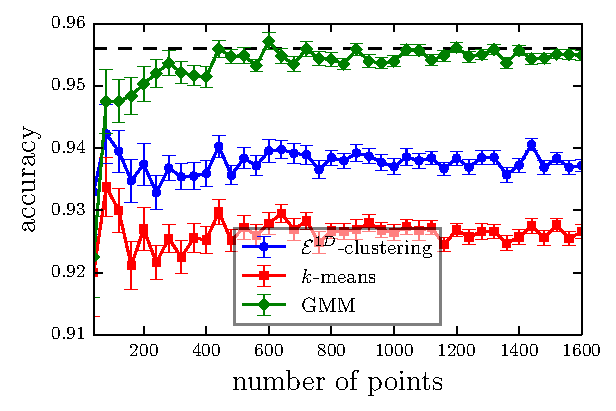
\includegraphics[width=\textwidth]{1D_normal.pdf}\\[-1em](a)
\end{minipage}
\begin{minipage}{0.49\textwidth}
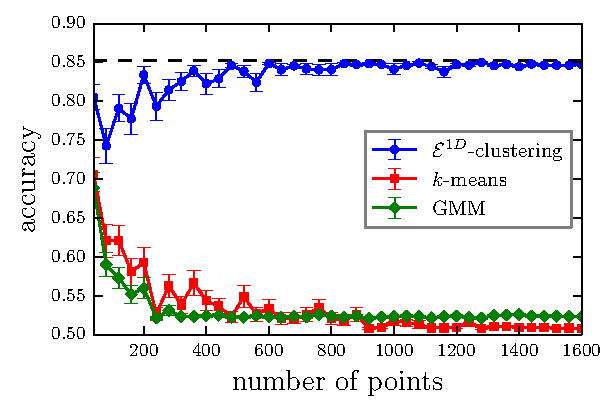
\includegraphics[width=\textwidth]{1D_lognormal.pdf}\\[-.8em](b)
\end{minipage}
\caption{
\label{fig:1d}
$\mathcal{E}^{1D}$-clustering versus $k$-means and GMM in one dimension.
The two clusters have the same number of points, and we use
$50$ Monte Carlo runs.
We plot the average 
accuracy \eqref{eq:accuracy} versus the total number of points, 
where error bars are standard error. The dashed line indicates 
Bayes accuracy. (a) Data distributed as \eqref{eq:two_normal}, where the
optimal accuracy is $\approx 0.956$.
(b) Data from \eqref{eq:two_lognormal} where the optimal
accuracy is $\approx 0.852$.
% @gui: if you insist on using the equations, at least also mention something semantic about them, ie, Data distributed Gaussian (as in 46), or Data distributed log Gaussian (as in 47).  figures & captions should stand on their own without requiring referring to the paper.
}
% @gui: why did you take away the plot of the distribution? those are incredibly helpful.  
\end{figure}

We now consider two simple experiments where we sample the same 
number of points for each cluster. 
We plot the average accuracy \eqref{eq:accuracy} versus the 
total number of points, with error bars indicating standard error.
The data is clustered using $\mathcal{E}^{1D}$-clustering algorithm,
GMM through EM algorithm, and the standard $k$-means 
algorithm. For $k$-means and GMM we use the implementations
from the well-known \emph{scikit-learn} library in 
Python \cite{scikit-learn}, where $k$-means is initialized through
$k$-means++ procedure \cite{Vassilvitskii}, and GMM is initialized
with the output of $k$-means. We choose to run both algorithms
$5$ times with different initializations and the answer with best 
objective function value is returned.
Notice that $\mathcal{E}^{1D}$-clustering does not require any random
initialization so we only run it once.
For each fixed number of points we use use $50$ Monte Carlo runs.
In  Fig.~\ref{fig:1d}a 
we have the results for data sampled from two normal distributions, 
\begin{equation}
\label{eq:two_normal}
x \sim \mathcal{N}\big(\mu_i,\sigma_i^2\big) 
\quad 
\mbox{with $\mu_1 = 0$, $\sigma_1=1$ and
$\mu_2 = 5$, $\sigma_2 = 2$.}
\end{equation}
In this case the optimal accuracy 
obtained from Bayes classification error
is $ \approx 0.956$, indicated by the dashed line in the plot.
The three methods
perform closely, with a slight advantage of GMM, as expected since
it corresponds to the true model of the data, and
$\mathcal{E}^{1D}$-clustering performs slightly better
than $k$-means. On the other hand, in Fig.~\ref{fig:1d}b
we consider two clusters with lognormal distributions,
\begin{equation}
\label{eq:two_lognormal}
\log x \sim \mathcal{N}\big( \mu_i,\sigma_i^2\big) \quad
\mbox{with
$\mu_1 = 0$,
$\sigma_1 = 0.3$ and
$\mu_2 = -1.5$,
$\sigma_2 = 1.5$.}
\end{equation}
The optimal classification accuracy from Bayes error is $\approx 0.852$.
We can now see that $\mathcal{E}^{1D}$-clustering
is still  very accurate, while
GMM and $k$-means basically cluster at chance.
The two simple experiments of Fig.~\ref{fig:1d} illustrate
how energy statistics does not make assumptions about the distributions
of the data, providing more flexibility and being able
to accurately cluster data with very different distributions.


%%%%%%%%%%%%%%%%%%%%%%%%%%%%%%%%%%%%%%%%%%%%%%%%%%%%%%%%%%%%%%%%%%%%%%%%%%%%%%%
\section{Iterative Algorithms for Energy Clustering}
\label{sec:algo}

In this section we introduce an iterative algorithm to find a local
maximizer of the optimization problem \eqref{eq:qcqp2}. Due to 
Proposition~\ref{th:kernel_kmeans} we can also find an approximate
solution by the well-known kernel $k$-means algorithm based
on Lloyd's heuristic (see \cite{Dhillon2,Dhillon}), which 
for convenience will also be restated in the present context.

Consider the optimization problem 
written in the form \eqref{eq:max_prob} as follows:
\begin{equation}
\label{eq:maxQ}
\max_{\{ \C_1,\dotsc,\C_k \}} 
\bigg\{ Q = \sum_{j=1}^k \dfrac{Q_j}{n_j}  \bigg\},
\qquad Q_j \equiv \sum_{x,y\in\C_j} \kk(x,y),
\end{equation}
where $Q_j$ represents an internal energy cost of cluster $\C_j$, and
$Q$ is the total energy cost where each $Q_j$ 
is weighted by the inverse
of the number of points in $\C_j$. For a data point $x_i$ we denote
its own energy cost
with the entire cluster $\C_\ell$ by
\begin{equation}
\label{eq:costxij}
Q_\ell(x_i) \equiv \sum_{y\in\C_\ell} \kk(x_i, y) = 
G_{i \bullet} \cdot Z_{\bullet \ell},
\end{equation}
where we recall that $G_{i\bullet}$ ($G_{\bullet i}$) denotes
the $i$th row (column) of matrix $G$.


\subsection*{Lloyd's Method for Energy Clustering}

To optimize the kernel $k$-means objective function
\eqref{eq:J} we remove the global term and define the function
\begin{equation}
\label{eq:Jell}
J^{(\ell)}(x_i) \equiv 
\dfrac{1}{n_\ell^2} Q_\ell
-\dfrac{2}{n_\ell} Q_\ell(x_i) .
\end{equation}
We are thus solving 
\begin{equation}
\min_{Z} 
\sum_{i=1}^n 
\sum_{\ell=1}^k Z_{i\ell} J^{(\ell)}(x_i).
\end{equation}
One possible strategy is to
assign  $x_i$ to cluster $\C_{j^\star}$ according
to 
\begin{equation}
j^\star = \argmin_{\ell=1,\dotsc,k} J^{(\ell)}(x_i) .
\end{equation}
This is done for every data point $x_i$ and repeated until
convergence, i.e. until no new assignments are made.
The entire procedure is described in Algorithm~\ref{kmeans_algo}, which
we name $\mathcal{E}^L$-clustering to emphasize
that we are optimizing the withn energy function $W$ 
based on Lloyd's method \cite{Lloyd}.
It can be shown that this algorithm converges provided $G$ is positive
semidefinite. 

% @jovo: check this paragraph. I included it to answer your question
% about having K(x,x) and \ell=1,...,k without exluding \ell=j. Essentially,
% the term K(x,x) will be hidden inside the mean of the cluster to which
% x is currently assigned to. This also clarifies the connection to 
% the standard formulation of kernel k-means.
$\mathcal{E}^{L}$-clustering is precisely
kernel $k$-means algorithm \cite{Dhillon2,Dhillon} 
but written more concisely and with the kernel induced by energy statistics. Indeed, recalling that
$\kk(x,y)=\langle \varphi(x), \varphi(y) \rangle$ where $\varphi: \mathcal{X}
\to \mathcal{H}_\kk$ is the feature map, we have from \eqref{eq:Jell} that
\begin{equation}
%\begin{split}
J^{(\ell)}(x_i) 
%&= \dfrac{1}{n_\ell^2} \sum_{x, y \in \C_\ell} 
%\langle \varphi(x), \varphi(y) \rangle - \dfrac{2}{n_\ell}
%\sum_{y\in \C_\ell} \langle \varphi(x_i), \varphi(y)\rangle \\ 
= 
\langle \varphi(\mu_\ell), \varphi(\mu_\ell) \rangle
-2 \langle \varphi(x_i), \varphi(\mu_\ell) \rangle 
= 
\| \varphi(x_i) - \varphi(\mu_\ell) \|^2 - \| \varphi(x_i) \|^2,
%\end{split}
\end{equation}
where $\mu_\ell = \tfrac{1}{n_\ell} \sum_{x\in \C_\ell}x$ 
is the mean of cluster $\C_\ell$. 
Therefore, $\min_\ell J^{(\ell)}(x_i) = 
\min_\ell \| \varphi(x_i) - \varphi(\mu_\ell)\|^2$, i.e. we are assigning
$x_i$ to the cluster with closest center (in feature space),
which is the familiar Lloyd's
heuristic approach that kernel $k$-means is based upon.

To check the complexity of $\mathcal{E}^L$-clustering, 
notice that to compute the second term of $J^{(\ell)}(x_i)$
in \eqref{eq:Jell} requires
$\OO(n_\ell)$ operations, and although the first term requires
$\OO(n_\ell^2)$ it only needs to be computed once outside loop through
data points (step 1 of Algorithm~\ref{kmeans_algo}).
Therefore, the time complexity of $\mathcal{E}^L$-clustering 
is
$\OO(n k \max_\ell n_\ell) = \OO(k n^2)$. For a sparse
Gram matrix $G$ having
$n'$ nonzero elements this complexity can be further reduced
to $\OO(k n')$. 

\begin{figure}
\begin{flushleft}
\begin{algorithm}[H]
\vspace{.5em}
\begin{algorithmic}[1]
    \INPUT number of clusters $k$, Gram matrix $G$, initial label
    matrix $Z \leftarrow Z_0$
    \OUTPUT label matrix $Z$ 
  \STATE $q \leftarrow (Q_1, \dotsc, Q_k)^\top$ 
            have the costs of each cluster, defined in \eqref{eq:maxQ}
  \STATE $n \leftarrow (n_1,\dotsc,n_k)^\top$ 
        have the number of points in each cluster%, obtained 
        %from $D = Z^\top Z$
  \REPEAT
    \FOR{ $i=1,\dotsc,n$}
        \STATE let $j$ be such that $x_i \in \C_j$
        \STATE $j^\star \leftarrow \argmin_{\ell=1,\dotsc,k} J^{(\ell)}(x_i)$,
            where $J^{(\ell)}(x_i)$ is defined in \eqref{eq:Jell}
            %, for $\ell=1,2,\dots,k$
        \IF{ $j^\star \ne j$} 
            \STATE move $x_i$ to $\C_{j^\star}$: $Z_{ij} \leftarrow 0$ and
            $Z_{ij^\star} \leftarrow 1$
            \STATE update $n$: $n_j \leftarrow n_j - 1$ and
                    $n_{j^\star} \leftarrow n_{j^\star} + 1$
            \STATE update $q$: $q_j \leftarrow q_j - 2Q_j(x_i)$ and
    $q_{j^\star} \leftarrow q_{j^\star} + 2Q_{j^\star}(x_i)$
    %    \ELSE
    %        \STATE Do nothing;
        \ENDIF
    \ENDFOR
  \UNTIL{convergence}
\end{algorithmic}
\caption{\label{kmeans_algo}
$\mathcal{E}^{L}$-clustering is Lloyd's method for energy clustering, which
is precisely~~~~~~~~ \\ 
kernel $k$-means algorithm, with the kernel induced by energy statistics. This procedure finds
local solutions to the problem \eqref{eq:qcqp2}.\hspace{\fill}
% @gui: spacing is weird.
}
\end{algorithm}
\end{flushleft}
\end{figure}

\subsection*{Hartigan's Method for Energy Clustering}

% @jovo: I also clarified this section, specially the derivation
% of the algorithm. Actually there was a mistake in the previous formula,
% which carried over to my code. Now it's fixed and better.

We now consider Hartigan's method \cite{Hartigan} 
applied to the optimization problem in the form \eqref{eq:maxQ}, which gives
a local solution to the QCQP defined in \eqref{eq:qcqp2}. 
The method is based in computing the maximum change
in the total cost function $Q$ when moving each data point to
another cluster. More specifically, 
suppose point $x_i$
is currently assigned to  cluster $\C_j$ yielding
a total cost function denoted by $Q^{(j)}$.
Moving $x_i$ to cluster $\C_\ell$ yields another total cost function
denoted by $Q^{(\ell)}$. We are interested in computing the maximum 
cost change
$\Delta Q^{j\to \ell} (x_i) \equiv Q^{(\ell)} - Q^{(j)}$, for $\ell\ne j$. 
From \eqref{eq:maxQ}, by explicitly writing the costs related to these 
two cluster we obtain
\begin{equation}
\Delta Q^{j\to \ell} (x_i) = \dfrac{Q_\ell^{+}}{n_\ell+1} + 
\dfrac{Q_j^-}{n_j-1} - \dfrac{Q_j}{n_j} - \dfrac{Q_\ell}{n_\ell}
\end{equation}
where $Q^{+}_\ell$ denote the cost of the new $\ell$th cluster
with the point $x_i$ added to it, and $Q^-_j$ is the cost of new 
$j$th cluster with $x_i$ removed from it. Noting that 
$Q_\ell^{+} = Q_\ell + 2 Q_\ell(x_i) + G_{ii}$ and
$Q_j^{-} = Q_j - 2 Q_j(x_i) + G_{ii}$, we get the formula
\begin{equation}
\label{eq:changeQ}
\Delta Q^{j \to \ell}(x_i)  = 
\dfrac{1}{n_j - 1}\left[ \dfrac{Q_j}{n_j} - 2 Q_j(x_i) + G_{ii} \right]
- \dfrac{1}{n_\ell + 1}\left[ \dfrac{Q_\ell}{n_\ell} - 2 Q_\ell(x_i) 
- G_{ii} \right].
\end{equation}
Therefore, if $\Delta Q^{j\to \ell}(x_i) > 0$ we get closer to a 
maximum of \eqref{eq:maxQ} by
moving $x_i$ to $\C_\ell$, otherwise we keep $x_i$ in $\C_j$. 

We thus propose an algorithm that goes as follows.
We start with an initial configuration for the label matrix $Z$, 
then for each
point $x_i$ 
we compute the cost of moving it to another cluster $\C_\ell$, i.e.
$\Delta Q^{j\to \ell}(x_i)$ for 
$\ell=1,\dots,k$ with $\ell \ne j$, where $j$ denotes the index of its current
partition, $x \in \C_j$. Hence, we choose
\begin{equation}
j^\star = \argmax_{\ell=1,\dotsc,k \, | \, \ell\ne j} 
\Delta^{j \to \ell}(x_i).
\end{equation}
If $\Delta Q^{j \to j^\star}(x_i) > 0$ 
we move $x_i$ to cluster $\C_{j^\star}$, otherwise 
we keep $x_i$ in its original cluster $\C_j$. 
This process is repeated
until no points are assigned to new clusters. 
The entire procedure is explicitly described in Algorithm~\ref{algo}, which we
denote $\mathcal{E}^H$-clustering to emphasize that it is based on
Hartigan's method.
This method automatically ensures that the objective function is
monotonically increasing at each iteration, and consequently the algorithm
converges in a finite number of steps.

\begin{figure}
\begin{flushleft}
\begin{algorithm}[H]
\vspace{.5em}
\begin{algorithmic}[1]
    \INPUT number of clusters $k$, Gram matrix $G$, 
                initial label matrix $Z \leftarrow Z_0$
    \OUTPUT label matrix $Z$
  \STATE $q \leftarrow (Q_1, \dotsc, Q_k)^\top$ 
            have the energy costs of each cluster, defined in \eqref{eq:maxQ}
  \STATE $n \leftarrow (n_1,\dotsc,n_k)^\top$ have the number of points 
        in each cluster%, obtained from $D=Z^\top Z$
  \REPEAT
    \FOR{ $i=1,\dotsc,n$}
        \STATE let $j$ be such that $x_i \in \C_j$
        \STATE $j^\star \leftarrow \argmax_{\ell=1,\dotsc,k \, | \, \ell\ne j} 
                \Delta Q^{j\to \ell}(x_i)$
            %for $\ell=1,2,\dots,k$ and $\ell \ne j$; 
            using \eqref{eq:changeQ} \label{stepmove}
        \IF{ $\Delta Q^{j \to j^\star}(x_i) > 0$ }
            \STATE move $x_i$ to $\C_{j^\star}$: $Z_{ij} \leftarrow 0$ and 
            $Z_{ij^\star} \leftarrow 1$
            \STATE update $n$: $n_j \leftarrow n_j - 1$ and
                    $n_{j^\star} \leftarrow n_{j^\star} + 1$
            \STATE update $q$: $q_j \leftarrow q_j - 2Q_j(x_i) + G_{ii}$ and
    $q_{j^\star} \leftarrow q_{j^\star} + 2Q_{j^\star}(x_i)+ G_{ii}$
    %    \ELSE
    %        \STATE Do nothing;
        \ENDIF
    \ENDFOR
  \UNTIL{convergence}
\end{algorithmic}
\caption{\label{algo}
$\mathcal{E}^H$-clustering is Hartigan's method for energy clustering.
This algorithm~~~~~~ \\ finds local solutions to  
the optimization problem \eqref{eq:qcqp2}.\hspace{\fill}
% @gui: clarify precisely which steps are different from alg 3 in caption.
\hspace{\fill}
}
\end{algorithm}
\end{flushleft}
\end{figure}

The complexity analysis of $\mathcal{E}^H$-clustering is the following.
Computing the Gram matrix $G$ requires $\OO( D n^2)$ operations, where 
$D$ is the dimension of each data point and $n$ is the data size. However,
both algorithms $\mathcal{E}^L$- and $\mathcal{E}^H$-clustering 
assume that $G$ is given. There are more efficient
methods to compute $G$, specially if it is sparse, but we will not consider
this further and just assume that $G$ is given.
The computation of each cluster cost
$Q_j$ has complexity $\OO(n_j^2)$, and overall to compute $q$
we have $\OO(n_1^2+\dots + n_k^2) = \OO(k \max_j n_j^2)$. 
These operations only need to be performed a single time. For
each point $x_i$ we need to compute $Q_j(x_i)$ once, which is
$\OO(n_j)$, and we need to compute $Q_\ell(x_i)$ for each $\ell\ne j$. 
The cost of computing 
%\eqref{eq:costxij} 
$Q_\ell(x_i)$
is $\OO(n_\ell)$, thus the cost of step~$6$ in
Algorithm~\ref{algo} is $\OO(k \max_\ell n_\ell)$ for $\ell=1,\dotsc,k$.
For the 
entire dataset this gives a time complexity
of $\OO(n k  \max_\ell n_\ell) =\OO(k n^2)$. Note that this is the same cost as
in $\mathcal{E}^L$-clustering, or kernel $k$-means algorithm. 
Again, if $G$ is sparse
this can be reduced to $\OO(k n')$ where $n'$ is the number of nonzero
entries of $G$.

In the following we mention some important known 
results about Hartigan's method.

\begin{theorem}[Telgarsky-Vattani \cite{Telgarsky}]
Hartigan's method has the cost function strictly decreasing in each
iteration. Moreover, if $n > k$ then 
\begin{enumerate}
\item \label{noempty} the resulting partition has no empty clusters, and
\item \label{diffmean} the resulting partition has distinct means.
\end{enumerate}
\end{theorem}

Neither of these two conditions are guaranteed to be 
satisfied  by Lloyd's method,
and consequently by $\mathcal{E}^L$-clustering 
algorithm.
The next result indicates that Hartigan's method can potentially 
escape local optima of Lloyd's method.

\begin{theorem}[Telgarsky-Vattani \cite{Telgarsky}]
The set of local optima of Hartigan's method is a (possibly strict) subset
of local optima of Lloyd's method.
\end{theorem}

The above theorem implies that $\mathcal{E}^L$-clustering  cannot
improve on a local optima of $\mathcal{E}^H$-clustering. On the other hand,
$\mathcal{E}^H$-clustering might improve on a local optima of 
$\mathcal{E}^L$-clustering. Lloyd's method forms Voronoi partitions,
while Hartigan's method groups data
in regions formed by the intersection of spheres called circlonoi cells.
It can be shown that the circlonoi cells are contained within
a smaller volume of a Voronoi cell, and this excess volume grows
exponentially with the dimension of $\mathcal{X}$ 
\cite[Theorems 2.4 and 3.1]{Telgarsky}. 
Points in this excess volume
force Hartigan's method to iterate, contrary
to Lloyd's method. Therefore, Hartigan's 
can escape local
optima of Lloyd's. 
Moreover, this improvement should be more prominent as
dimension increases. Also, the improvement grows as the number of clusters
$k$ increases.
The empirical results of \citet{Telgarsky} show that 
an implementation of Hartigan's method has comparable execution time 
to an implementation of
Lloyd's method,
but no explicit complexity was provided. We show that both
$\mathcal{E}^L$- and $\mathcal{E}^H$-clustering
have the same time complexity. To the best of our knowledge, Hartigan's
method was not previously considered together with kernels, as we 
are proposing
in $\mathcal{E}^{H}$-clustering.

% @gui: if you refer to a manuscript, it is not usually acceptable to just write the number. for example, sometimes the numbers are superscripts.  citet should work.
In \citet{Slonin}, Hartigan's method was applied to $k$-means problem
with any Bregman divergence. It was shown that the number of Hartigan's
local optima is upper bounded by $\mathcal{O}(1/k)$ 
\cite[Proposition 5.1]{Slonin}. 
In addition, it was provided examples where
\emph{any} initial partition correspond to a local optima of Lloyd's 
method, while  the number of local optima in Hartigan's method is small and 
correspond to true partitions of the data. Empirically, the number of
Hartigan's local optima was considerably smaller than the number of Lloyd's
local optima.

The above results indicate that Hartigan's method
provides several advantages over Lloyd's method, a fact that will also
be supported by our numerical experiments in the next section where 
$\mathcal{E}^H$-clustering  outperforms
of $\mathcal{E}^L$-clustering (kernel $k$-means) in several settings,
specially in high dimensions.


%%%%%%%%%%%%%%%%%%%%%%%%%%%%%%%%%%%%%%%%%%%%%%%%%%%%%%%%%%%%%%%%%%%%%%%%%%%%%%%
\section{Numerical Experiments}
\label{sec:numerics}

% @gui: something is weird with the way you care computing accuracy.  GMM should not be significantly worse than chance.  i think you are probably counting the NaN's as *wrong*, rather than nothing?
% now I'm using GMM from sklearn which eliminated previous weird things.
% I think my method was too crude and the covariance estimate was too bad in
% some cases

% @gui: i'm not convinced you need alg 2 in these tables at all. if i were to add alg 2 to these tables, however, i would do the same thing i would for the figs, that is, for each simulation, compute the diff between performance on alg 2 and alg 3, and report that.
% @jovo: yes I agree. I included new plots in the fig, but didn't do anything
% for the tables cuz I don't think necessary

% @jovo: added this paragraph
The main goal of this section is threefold. First, we want to compare
energy clustering, based on the kernels provided by the standard energy
distance $\mathcal{E}_\alpha$, to $k$-means and GMM. Second, we want
to compare $\mathcal{E}^H$-clustering, based on Hartigan's method, to
$\mathcal{E}^L$-clustering, based on Lloyd's method. We also compare
to $\mathcal{E}^S$-clustering
which is an exact solution to the relaxed problem.
Third, we want to illustrate the flexibility
provided by energy clustering which do not make assumptions about the
distribution of the data, being able to cluster accurately in different
settings while keeping the same standard kernel.

In the experiments below we fix the semimetric 
according to the traditional energy distance, $\alpha=1$, and
the point $x_0=0$ is chosen in the corresponding kernel  
\eqref{eq:kernel_semimetric}. We thus have
\begin{equation}
\label{eq:standard_metric}
\rho(x,y) = \| x-y\| \qquad \mbox{and} \qquad \kk(x,y) = 
\tfrac{1}{2}\left( \| x \| + \| y \| - \| x-y \| \right).
\end{equation}
We shall consider other kernels as well, 
but \eqref{eq:standard_metric} will be the
standard kernel for energy statistics and will always be present in the
experiments as a reference.

We briefly mention that we compared $\mathcal{E}^H$-clustering,
as described in Algorithm~\ref{algo}, to
$\mathcal{E}^{1D}$-clutering, described in Algorithm~\ref{algo1d}, 
for several univariate distributions.
Both perform almost indistinguishable regarding the clustering quality.
However, we omit these results since we will analyse more interesting 
scenarios in high dimensions.

From the results of \cite{Telgarsky}, summarized in the end of the previous
section, we expect the improvement of Hartigan's 
over Lloyd's method to be more accentuated in high dimensions.
Thus, we analyze
how the algorithms degrade as the number of dimensions increase while
keeping the number of points in each cluster fixed.
Consider
two clusters with multivariate normal distributions given by
\begin{equation}
\label{eq:gauss1}
\begin{split}
x &\in \C_i  \sim 
\mathcal{N}(\mu_i,\Sigma_i) \qquad (i=1,2),  \\
\mu_1 &= (\underbrace{0,\dotsc,0}_{\times D})^\top , \quad
\mu_2 = 0.7 \times (\underbrace{1,\dots,1}_{\times 10},
\underbrace{0,\dots,0}_{\times (D-10)})^\top, \quad
\Sigma_1 = \Sigma_2 = I_D.
\end{split}
\end{equation}
Note that the Bayes error
is fixed as $D$ increases, yielding an optimal 
accuracy of $\approx 0.86$.
For each $D$ we generate $100$ Monte Carlo runs, 
sampling $100$ points for each cluster.
We apply each algorithm to the resulting dataset 
and compute the accuracy \eqref{eq:accuracy}. The algorithms
$\mathcal{E}^H$- and $\mathcal{E}^L$-clustering
both use the standard
kernel \eqref{eq:standard_metric}, as well as the spectral
$\mathcal{E}^S$-clustering method\footnote{We
compared our implementation of spectral clustering provided in
Algorithm~\ref{spectralalgo} with the spectral clustering routine provided
by \emph{scikit-learn} library \cite{scikit-learn}, 
which is based on \cite{Malik}. In the few
cases considered the algorithms had similar performance.
% @gui: dude, this is a crazy sentence to write. use sklearn, or have a *very* good reason not to.  
% currently, you utterly fail to justify the difference.
}, 
and we initialize the algorithms
with the initialization of $k$-means++ \cite{Vassilvitskii}.
% @gui: i thought you were goign to initialize E-H & E-L with E-S?
% @gui: you gotta clearly define E-S, with a pseudocode block, just like the others.  in particular, which matrix are you doing an eigendecomposition on, and how you are choosing the number of dimensions to embed into.
For $k$-means and GMM we use the implementation of \emph{scikit-learn} library
\cite{scikit-learn}, where $k$-means is also initialized with $k$-means++,
while GMM is initialized with the output of $k$-means. Every algorithm
is ran $5$ times, returning the answer with best objective function value.
We plot the average accuracy versus $D$, with error bars indicating
standard error.
The results are shown in Fig.~\ref{fig:gauss}a. We can see that
$\mathcal{E}^H$- and $\mathcal{E}^S$-clustering have practically
the same performance, which is 
much higher than $\mathcal{E}^L$-clustering (kernel
$k$-means). Moreover, $\mathcal{E}^H$-clustering outperforms 
$k$-means and GMM, where the improvement is noticeable specially in 
high dimensions.
Note that in this setting $k$-means and GMM are consistent estimators,
however, energy clustering degrades much less as dimension increases.
% @gui: k-means is only consistent if the prob of each class is equal.  but you did not actually define this parameter, because you sampled 100 from each.  so, you gotta define the parameter at least if you want to say anythng about consistency.  also, what do you mean k-means is a consistent estimator? estimator of what? clarify.

\begin{figure}
\begin{minipage}{0.49\textwidth}
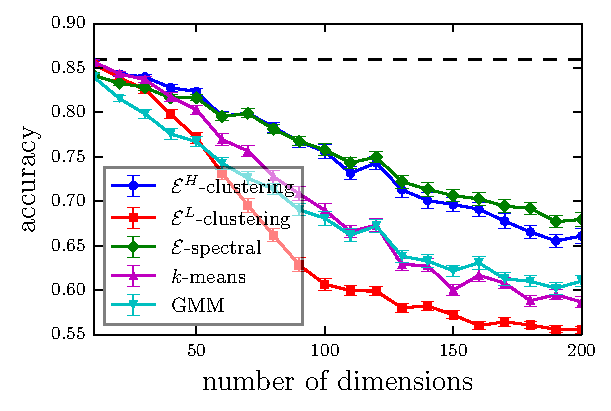
\includegraphics[width=1\textwidth]{normal_highdim_mean.pdf}\\[-1.0em] (a)
\end{minipage}
\begin{minipage}{0.49\textwidth}
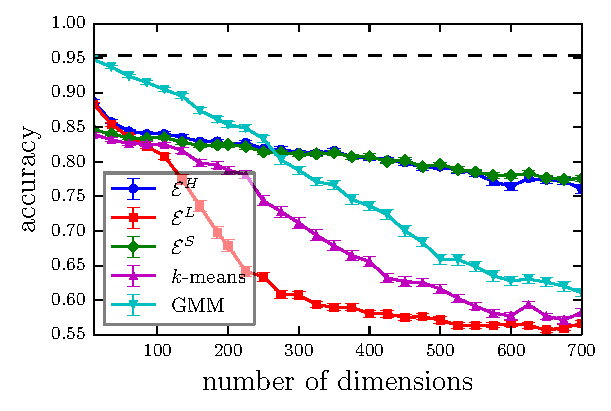
\includegraphics[width=1\textwidth]{normal_highdim_cov.pdf}\\[-1.0em] (b)
\end{minipage}
\caption{
\label{fig:gauss}
Comparison of energy clustering algorithms to $k$-means and GMM in 
high dimensional Gaussian settings. We plot the mean accuracy versus
the number of dimensions, with error bars indicating standard 
error from $100$ Monte
Carlo runs.
(a) Data distributed as in \eqref{eq:gauss1}, with Bayes
accuracy $\approx 0.86$, over the range $D \in [10,200]$. 
(b) Data distributed
as in \eqref{eq:gauss2}, with Bayes accuracy $\approx 0.95$,
over the range $D \in [10, 700]$.
% @gui: also helpful here would be pairs plots, say, of the first 5 dimensions, showing the performance of our stuff (color points by Alg 3, maybe symbols denote "truth".  i have no intuition how difficult these are.
% @jovo: didn't understand this
% @gui: https://www.google.com/search?q=pairs+plots&rlz=1C5CHFA_enUS731US731&source=lnms&tbm=isch&sa=X&ved=0ahUKEwjwo9u5w-DWAhXMKyYKHYkhAKMQ_AUICigB&biw=1440&bih=776
% to show how well separated the classes are.
}
\end{figure}

% @gui: for eq 59, E-H & E-S yield the same performance.  but for eq 63, E-H is much better than E-S.  do you have any idea why that is?
We now allow the diagonal covariance of the second Gaussian distribution to
have different values by choosing
$(\Sigma_2)_{ii} \stackrel{iid}{\sim} \textnormal{Uni}(1,5)$ for
$i=1,\dotsc,10$, and $(\Sigma_2)_{ii} = 1$ for $i=11,\dotsc,D$. For instance,
we consider the fixed setting
\begin{equation}
\label{eq:gauss2}
\begin{split}
x & \in \C_i  \sim 
\mathcal{N}(\mu_i,\Sigma_i) \quad (i=1,2),  \\
\mu_1 &= (\underbrace{0,\dotsc,0}_{\times D})^\top , \quad
\mu_2 = (\underbrace{1,\dots,1}_{\times 10},
\underbrace{0,\dots,0}_{\times (D-10)})^\top, \quad
\Sigma_1 = I_D, \quad
\Sigma_2 = \left( \begin{array}{c|c}
\widetilde{\Sigma}_{10} & 0 \\ \hline 
0 & I_{D-10} \end{array}\right), \\
\widetilde{\Sigma}_{10} &= \diag(1.367,  3.175,  3.247,  4.403,  1.249,
1.969, 4.035,   4.237,  2.813,  3.637),
\end{split}
\end{equation}
as we vary $D$. Note that there is nothing special about the numbers in
$\widetilde{\Sigma}_{10}$, it is simply a random choice of sampling
$\textnormal{Uni}(1,5)$ ten times, and one could pick any other choices
as well.
% @gui: if there is nothing special, why not just use 2*ones?  this seems suspicious.  also, it is the result of sampling 1 time, not 10 times.
The Bayes error is kept fixed yielding
an optimal accuracy $\approx 0.95$.
% @gui: bayes error changes for each random sample, unless you are integrating over all possible samples?  it is not fixed.
In Fig.~\ref{fig:gauss}b we show the results of energy clustering,
$k$-means, and GMM.
Note that GMM performs better in low dimensions, 
since it is a consistent estimator.
However, $\mathcal{E}^H$ and $\mathcal{E}^S$ degrade much less as dimensions
increase, performing better than $k$-means and GMM in high dimensions.
% @gui: you gotta explain why GMM doesn't utterly fail when D>n!
 
 % @gui: maybe put this below section in the discussion?
Consider the effect of having 
unbalanced clusters according to
\begin{equation}
\label{eq:gauss3}
\begin{split}
x &\in \C_i \sim  
\dfrac{n_i}{N} \mathcal{N}(\mu_i,\Sigma_i) \quad (i=1,2), \quad 
\mu_1 = (0,0,0,0)^\top , \quad
\mu_2 = 1.5\times (1,1,0,0)^\top, \\
\Sigma_1 &= I_4, \quad
\Sigma_2 = \left( 
\begin{array}{c|c} 
\tfrac{1}{2} I_2 & 0  \\ \hline
0 & I_2 
\end{array}\right), \quad
n_1 = N - m, \quad  n_2 = N + m, \quad N=250.
\end{split}
\end{equation}
We then increase $m \in [0,240]$ making
the clusters progressively more unbalanced.
We plot the average accuracy over
$100$ Monte Carlo runs for each $m$, with error bars indicating 
standard error. 
The results are shown in Fig.~\ref{fig:unbalanced}.
For highly unbalanced clusters we see that GMM performs better than
the other methods, which have basically similar performance.
Based on this experiment, an interesting problem would be to
extend $\mathcal{E}^H$-clustering algorithm to account for 
highly unbalanced clusters.

\begin{figure}
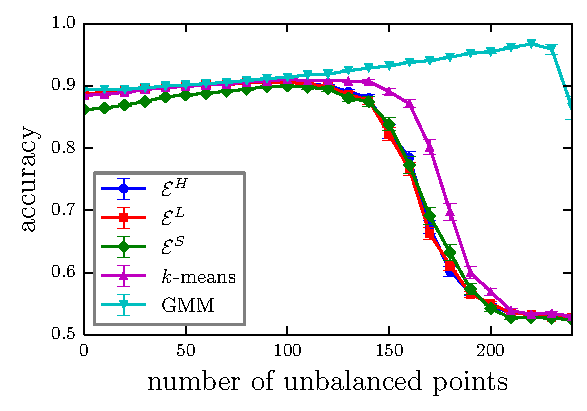
\includegraphics[width=0.5\textwidth]{normal_unbalanced.pdf}\vspace{-1em}
\caption{
\label{fig:unbalanced}
Comparison of energy clustering algorithms to $k$-means and GMM on
unbalanced clusters. The data is distributed as \eqref{eq:gauss3}, where
we vary $m \in [0, 240]$, and in each case we do $100$ Monte Carlo runs
showing the average accuracy with standard error.
}
\end{figure}

Besides the standard kernel from energy statistics 
\eqref{eq:standard_metric}, 
consider the following two other semimetrics with their respective generating
kernels:
\begin{align}
\rho_{1/2}(x,y) &= \| x-y \|^{1/2} & 
 \kk_{1/2}(x,y) &= \tfrac{1}{2} \left( 
\| x \|^{1/2} + \| y \|^{1/2} 
- \| x-y \|^{1/2} \right), \label{eq:rhohalf}\\
\rho_{e}(x,y) &= 
2 - 2 e^{-\tfrac{1}{2}\| x- y\|} &
 \kk_{e}(x,y) &= e^{-\tfrac{1}{2}\| x-y\|}.
\label{eq:rhoe}
\end{align}
The kernel $K_{1/2}(x,y)$ corresponds to the standard energy distance
with $\alpha=1/2$.
We sample data from the following normal distribution in $20$ dimensions:
\begin{equation}
\label{eq:20gauss}
\begin{split}
x &\in \C_i \sim \mathcal{N}(\mu_i,\Sigma_i) \qquad (i=1,2), \\
\mu_1 &= (\underbrace{0,\dotsc,0}_{\times 20})^\top ,\quad
\mu_2 = \tfrac{1}{2} 
(\underbrace{1,\dotsc,1}_{5},\underbrace{0,\dotsc,0}_{15})^\top, \quad
\Sigma_1 = \tfrac{1}{2} I_{20},  \quad
\Sigma_2 = I_{20}.
\end{split}
\end{equation}
The optimal accuracy based on Bayes
classification error is $\approx 0.90$. 
We sample an equal number of points for each cluster which is progressively
increased, $n \in [5, 200]$. 
The results over $100$ Monte Carlo trials are 
shown in Fig.~\ref{fig:consist}a, where we compare
$\mathcal{E}^H$-clustering, with different
kernels, to $k$-means and GMM.
Note that for small $n$ all methods
are superior than GMM, which slowly catches up and tend to optimal Bayes,
as expected since it is a consistent estimator in this case. 
Note also that $\mathcal{E}^H$-clustering
with kernel $\kk_e$ is as accurate as GMM for large number of points, however,
it is superior for small number of points. Still for
the same setting, in Fig.~\ref{fig:consist}b we
we show the difference in accuracy provided by $\mathcal{E}^H$ minus
$\mathcal{E}^L$ and $\mathcal{E}^S$, when using the
kernel $\kk_e$.
Note that $\mathcal{E}^H$ was
always superior than the other 
methods (there would be points negative values on the $y$-axis otherwise).

\begin{figure}
\begin{minipage}{0.49\textwidth}
\centering
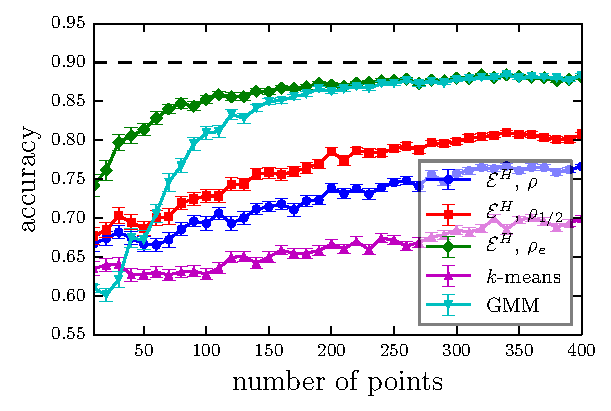
\includegraphics[width=1\textwidth]{normal_kernels.pdf}\\[-1.0em](a)
\end{minipage}
\begin{minipage}{0.49\textwidth}
\centering
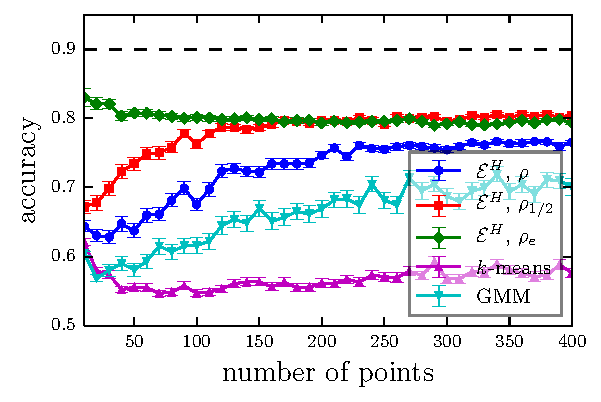
\includegraphics[width=1\textwidth]{lognormal_kernels.pdf}\\[-1.0em](c)
\end{minipage}
\begin{minipage}{0.49\textwidth}
\centering
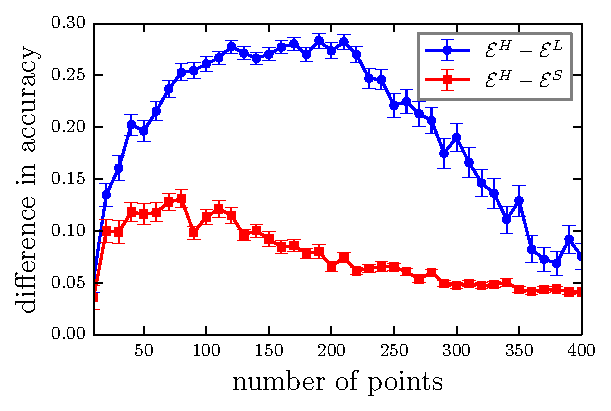
\includegraphics[width=1\textwidth]{normal_kernels_difference.pdf}\\[-1.0em](b)
\end{minipage}
\begin{minipage}{0.49\textwidth}
\centering
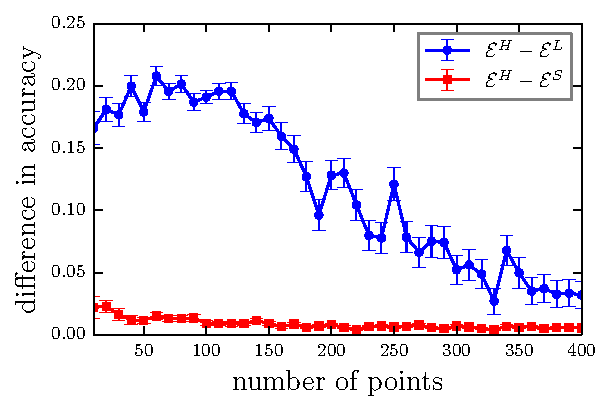
\includegraphics[width=1\textwidth]{lognormal_kernels_difference.pdf}\\[-1.0em]
(d)
\end{minipage}
\caption{
\label{fig:consist}
$\mathcal{E}^H$-clustering with different kernels versus
$k$-means and GMM. In both settings Bayes accuracy
is $\approx 0.9$. We show average accuracy (error bars are standard error)
versus number of points for $100$ Monte Carlo trials.
(a,b) Normal distribution \eqref{eq:20gauss}. 
(c,d) Lognormal distribution~\eqref{eq:20loggauss}.
The plots in (c) and (d) consider the difference in accuracy
between $\mathcal{E}^H$ versus $\mathcal{E}^L$ and
$\mathcal{E}^S$-clustering, with semimetric $\rho_e$.
}
\end{figure}

Now consider the same parameters as in \eqref{eq:20gauss} but with
lognormal distributions, 
\begin{equation}
\label{eq:20loggauss}
\log x \in \C_i \sim \mathcal{N}(\mu_i, \Sigma_i) \qquad (i=1,2).
\end{equation}
The same previous experiment is shown in 
Fig.~\ref{fig:consist}c.
Energy clustering still performs accurately, with any of the utilized
kernels, providing better results than $k$-means and GMM on
this non-normal data. The kernel $\kk_e$ still provides the best results
for small number of points, but its performance is eventually achieved by
$\kk_{1/2}$, indicating that $\alpha \approx 1/2$ in the standard
energy distance should be more appropriate for skewed distributions.
Still for the same setting, in Fig.~\ref{fig:consist}d
we show the difference in accuracy provided by $\mathcal{E}^H$ versus
$\mathcal{E}^L$ and $\mathcal{E}^S$, for the kernel $\kk_e$. Again,
the accuracy provided by $\mathcal{E}^H$ is higher than the other methods,
although not much higher than $\mathcal{E}^S$ in this example.
The two experiments of Fig.~\ref{fig:consist}
illustrate how energy statistics clustering does not make assumptions
about the distribution of the data, performing well in different settings
with the same kernel. 
% @gui: algs don't make assumptions.

\begin{figure}
\begin{minipage}{0.24\textwidth}
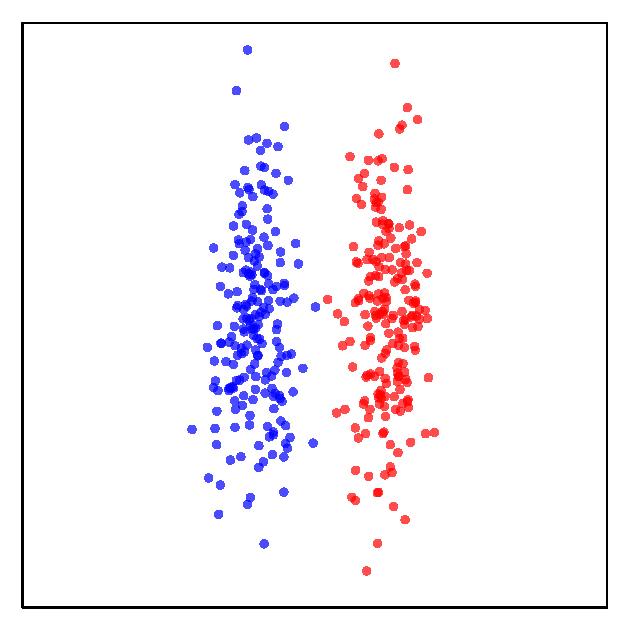
\includegraphics[width=1\textwidth]{2cigars.pdf}\\[-1em] (a)
\end{minipage}
\begin{minipage}{0.24\textwidth}
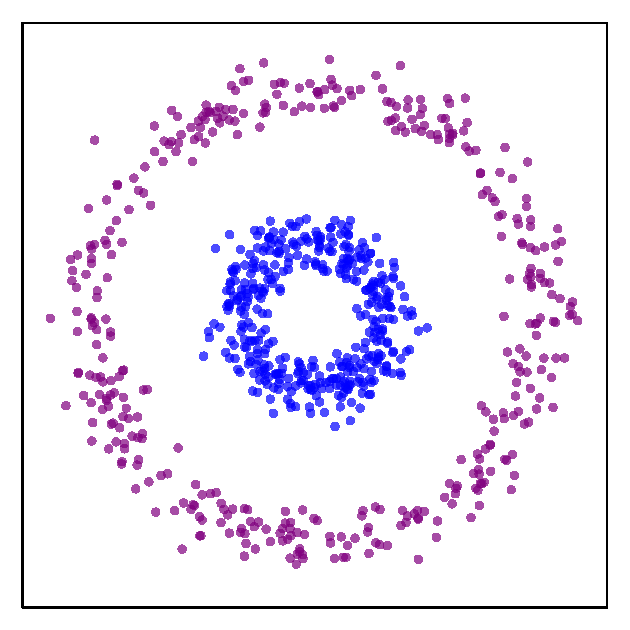
\includegraphics[width=1\textwidth]{2circles.pdf}\\[-1em] (b)
\end{minipage}
\begin{minipage}{0.24\textwidth}
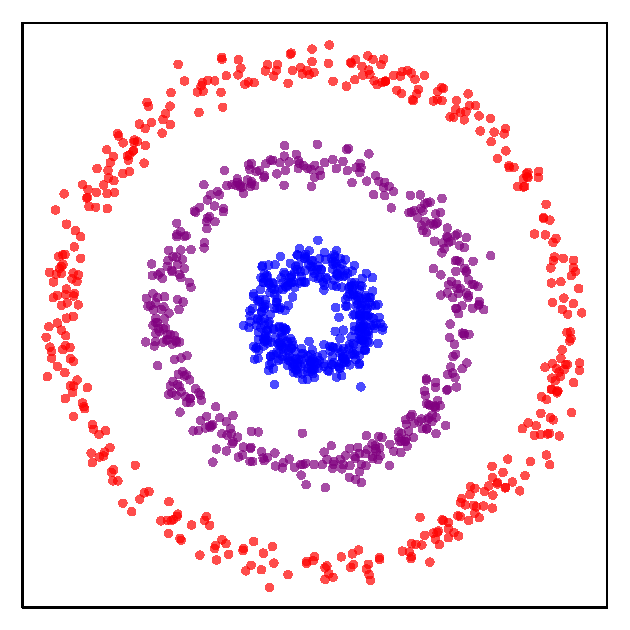
\includegraphics[width=1\textwidth]{3circles.pdf}\\[-1em] (c)  
\end{minipage}
\begin{minipage}{0.23\textwidth}
\vspace{-0.9em}
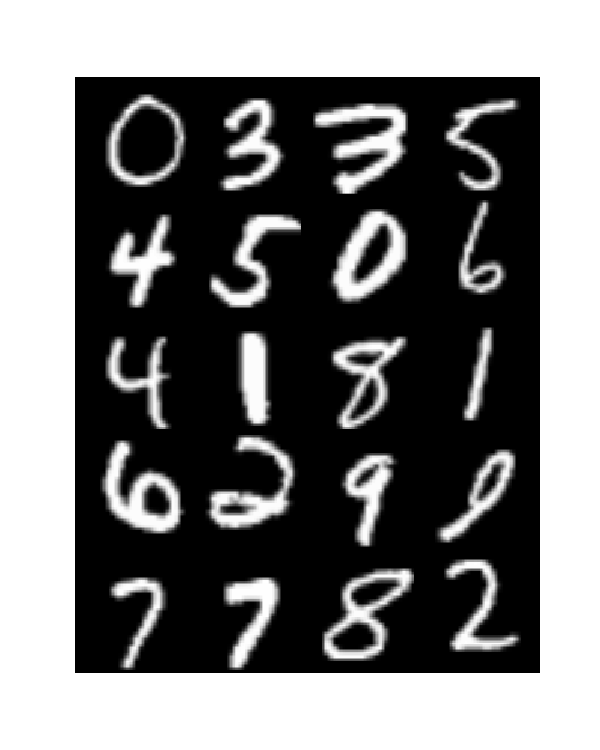
\includegraphics[width=1\textwidth]{mnist.pdf}\\[-1.8em] (d)  
\end{minipage}
\caption{\label{fig:other}
(a) Parallel cigars. (b) Two  
concentric circles with noise. (c) Three
concentric circles with noise. (d) MNIST handwritten digits.
Clustering results are in Table~\ref{table:other}
and Table~\ref{table:mnist}.
}
\end{figure}

Consider the following choices of semimetric and 
corresponding generating kernel:
\begin{align}
\rho_{\alpha}(x,y) &= \| x - y\|^\alpha & 
\kk_{\alpha}(x,y) &= \tfrac{1}{2}\left(
\| x \|^\alpha +
\| y \|^\alpha -
\| x-y \|^\alpha \right) ,
\label{eq:rhoalpha} \\
%
\widetilde{\rho}_{\sigma}(x,y) &= 2 - 2 e^{-\tfrac{\|x-y\|}{2 \sigma}} &
\widetilde{\kk}_{\sigma}(x,y) &= e^{-\tfrac{\|x-y\|}{2\sigma}} ,
\label{eq:rhoesigma} \\
%
\widehat{\rho}_{\sigma}(x,y) &= 2 - 2 e^{-\tfrac{\|x-y\|^2}{2 \sigma^2}} &
\widehat{\kk}_{\sigma}(x,y) &= e^{-\tfrac{\|x-y\|^2}{2\sigma^2}} .
\label{eq:rhogsigma} 
\end{align}
In Fig.~\ref{fig:other}a--c we have 
complex two dimensional datasets. The two parallel cigars in (a)
have $200$ points each. The concentric circles
in (b) and (c) have $400$ points for each class.
We apply $\mathcal{E}^H$-clustering  with different choices
of kernels in \eqref{eq:rhoalpha}--\eqref{eq:rhogsigma}. We also consider
the best kernel choice for each example for the spectral
$\mathcal{E}^S$-clustering. 
Moreover, we consider
$k$-means and GMM. We perform $10$ Monte Carlo runs for each example.
The results are in Table~\ref{table:other}.
%, where the respective 
%choice of parameters for the kernels are indicated. 
For (a) we initialize
all algorithms with $k$-means++, and for (b) and (c) we initialize at
random.
$\mathcal{E}^H$ has superior performance
in every example, and in particular better than the
spectral $\mathcal{E}^S$.
For the data in Fig.~\ref{fig:other}a 
the semimetrics $\rho_1$ and $\rho_{1/2}$ are
still able to provide accurate results, however, for the
examples in (b) and (c) the kernel choice is more sensitive.

\begin{table}[t]
\renewcommand*{\arraystretch}{0.75}
\begin{tabular}{@{}r  l g  l g  l g@{}}
\toprule[1pt]
 & & \emph{Fig.~\ref{fig:other}a}
 & & \emph{Fig.~\ref{fig:other}b}
 & & \emph{Fig.~\ref{fig:other}c} \\
\midrule[0.5pt]
\multirow{4}{*}{\emph{$\mathcal{E}^H$~~~~}}
& $\rho_{1}$ & $0.705\pm 0.065$
& $\rho_{1}$ & $0.521\pm 0.005$
& $\rho_{1}$ & $0.393\pm 0.020$ \\
& $\rho_{1/2}$ & $0.952\pm 0.048$
& $\rho_{1/2}$ & $0.522\pm 0.004$
& $\rho_{1/2}$ & $0.486\pm 0.040$ \\
& $\widetilde{\rho}_{2}$ & $\bm{0.9987\pm 0.0008}$
& $\widetilde{\rho}_{1}$ & $0.778\pm 0.075$
& $\widetilde{\rho}_{2}$ & $0.666\pm 0.007$ \\
& $\widehat{\rho}_{2}$  & $0.956\pm 0.020$
& $\widehat{\rho}_{1}$  & $\bm{1.0\pm 0.0}$
& $\widehat{\rho}_{2}$ & $\bm{0.676\pm 0.002}$ \\
\arrayrulecolor{gray!80}\midrule[0.5pt]
\emph{$\mathcal{E}^S$~~~~}
& $\widetilde{\rho}_{2}$ & $0.557\pm 0.014$ 
& $\widehat{\rho}_{1}$ & $0.732\pm 0.002$ 
& $\widehat{\rho}_{2}$ & $0.364\pm 0.004$  \\
\arrayrulecolor{gray!80}\midrule[0.5pt]
\emph{$k$-means}~~~~ 
& & $0.550\pm 0.011$
& & $0.522\pm 0.004$
& & $0.368\pm 0.005$ \\
\emph{GMM}~~~~
& & $0.903\pm 0.064$
& & $0.595\pm 0.011$
& & $0.465\pm 0.030$ \\
\arrayrulecolor{black}\bottomrule[1pt]
\end{tabular}
\caption{\label{table:other}
Clustering data from Fig.~\ref{fig:other}.
We show average
accuracy over $10$ Monte Carlo runs.
}
\end{table}

\begin{table}[t]
\renewcommand*{\arraystretch}{0.75}
\begin{tabular}{@{}r@{}l@{}|@{}l@{}|@{}l@{}|@{}l@{}|@{}l@{}}
\toprule[1pt]
\emph{Class Subset}~~~~ & & 
$~\{0,1,2\}$ &
$~\{0,1,\dotsc,4\}~$ &
$~\{0,1,\dotsc,6\}~$ &
$~\{0,1,\dotsc,8\}~$ \\
\midrule[0.5pt]
\multirow{3}{*}{\emph{$\mathcal{E}^H$-clustering~~~~}}
& $\rho_{1}$\hspace{1em} 
&$~0.937\pm 0.006~$
&$~0.873\pm 0.025~$
&$~0.731\pm 0.016~$
&$~0.687\pm 0.016~$
\\
& $\rho_{1/2}$ 
&$~0.939\pm 0.006~$
&$~0.874\pm 0.027~$
&$~0.722\pm 0.017~$
&$~0.647\pm 0.017~$
\\
& $\widetilde{\rho}_{\sigma}$ 
&$~0.939\pm 0.006~$
&$~0.847\pm 0.031~$
&$~0.695\pm 0.023~$
&$~0.657\pm 0.014~$
\\
& $\widehat{\rho}_{\sigma}$ 
&$~0.933\pm 0.005~$
&$~0.891\pm 0.009~$
&$~0.759\pm 0.011~$
&$~0.704\pm 0.011~$
\\
\arrayrulecolor{gray!80}\midrule[0.5pt]
\emph{$\mathcal{E}$-spectral~~~~} 
& $\widehat{\rho}_{\sigma}$ 
&$~0.823\pm 0.015~$
&$~0.769\pm 0.012~$
&$~0.678\pm 0.014~$
&$~0.649\pm 0.018~$
\\
\midrule[0.5pt]
\rowcolor{gray!20}
& {$\sigma$}
& $~10.34~$
& $~10.41~$
& $~10.41~$
& $~10.37~$
\\
\arrayrulecolor{gray!80}\midrule[0.5pt]
\emph{$k$-means}~~~~ &
&$~0.927\pm 0.004~$
&$~0.878\pm 0.010~$
&$~0.744\pm 0.008~$
&$~0.695\pm 0.012~$
\\
\arrayrulecolor{gray!80}\midrule[0.5pt]
\emph{GMM}~~~~ &
&$~0.952\pm 0.005~$
&$~0.839\pm 0.015~$
&$~0.694\pm 0.010~$
&$~0.621\pm 0.009~$
\\
\arrayrulecolor{black}\bottomrule[1pt]
\end{tabular}
\caption{\label{table:mnist}
Clustering MNIST data from Fig.~\ref{fig:other}d.
For each subset of digits we perform $10$ Monte Carlo runs, sampling 
$100$ points for  each class.
}
\end{table}

Next, we consider 
the infamous MNIST handwritten digits
as illustrated in Fig.~\ref{fig:other}d.
Each data point is an $8$-bit gray scale
image forming a $784$-dimensional vector 
corresponding to the digits $\{0,1,\dotsc,9 \}$.
Besides the kernel \eqref{eq:rhoalpha}, we
consider the Gaussian kernel \eqref{eq:rhogsigma} with 
\begin{equation}
\label{eq:sigma}
\sigma^2 = \dfrac{1}{n^2} \sum_{i,j=1}^n \| x_i - x_j \|^2 ,
\end{equation}
computed from a separate
training set.
We consider subsets of $\{0,1,\dotsc,9 \}$, 
sampling $100$ points 
for each class. 
% @gui: i don't understand these results. {0,1,2} we do worse.  why don't we show {0,1,...,9}?
% also, why don't you use a better metric/similarity designed for images? like using pairwise alignment followed by rho?
The results are shown in Table~\ref{table:mnist}, where kernels
and parameters are indicated.
$\mathcal{E}^H$-clustering performs slightly better than $k$-means
and GMM, however the difference is not considerable.
Unsupervised clustering on MNIST without any feature extraction
is not trivial. For instance,
the same experiment was performed in \cite{Sapiro} where a low-rank
transformation is learned then subsequently used in subspace clustering,
providing very accurate results. It would be interesting to 
explore analogous methods
for learning a better representation of the data and subsequently apply
$\mathcal{E}^H$-clustering.



%%%%%%%%%%%%%%%%%%%%%%%%%%%%%%%%%%%%%%%%%%%%%%%%%%%%%%%%%%%%%%%%%%%%%%%%%%%%%%%
\section{Discussion}
\label{sec:conclusion}

We considered clustering from the perspective of energy
statistics, which provides a non-parametric test for 
equality of distributions.
The mathematical formulation of energy clustering 
reduces to a QCQP in the associated RKHS, as demonstrated in 
Proposition~\ref{th:qcqp2}.
We showed that the optimization problem
is equivalent
to kernel $k$-means, once the kernel is fixed; see
Proposition~\ref{th:kernel_kmeans}. Energy statistics, however, fixes
a family of standard kernels in Euclidean space, and
more general kernels 
on semimetric spaces of negative type can also be obtained.
We also considered a weighted version of energy statistics, whose 
clustering formulation establishes connections with 
graph partitioning.
We proposed the iterative $\mathcal{E}^H$-clustering algorithm based on 
Hartigan's method, which was compared to kernel $k$-means algorithm
based on Lloyd's heuristic.
Both have the same time complexity, however, numerical and theoretical
results provide compelling evidence that $\mathcal{E}^H$-clustering
is more robust with a superior performance, specially in high
dimensions. 
Furthermore, energy clustering, with standard kernels from energy
statistics, outperformed $k$-means and GMM
on several settings, illustrating the flexibility
of the proposed method which is distribution-free. In many
settings, the iterative
$\mathcal{E}^H$-clustering also surpassed $\mathcal{E}^S$-clustering, which
is a spectral relaxation of the QCQP.

It would be interesting to formally 
demonstrate cases where energy clustering is a 
consistent estimator. A soft version of energy clustering is also an
interesting extension.
Finally, kernel methods can benefit from sparsity and
fixed-rank approximations of the Gram matrix, and there is plenty
of room to make $\mathcal{E}^H$-clustering algorithm more scalable.

% @gui: your discussion is basically just a summary, which i don't find very helpful to the reader.  if you want to summarize results, 1 paragraph is sufficient.  another paragraph connects it to previous work not already mentioned, and a third paragraph on additional possible extensions.  as you know, one thing i'd like to do next is to theoretically prove when Energy Clustering asymptoticaly gets the right answer. you also mentioned soft clustering, which is another potential extension, or incorporating this into subspace clustering.
% @jovo: not clear how to make the conclusion?
% how do you think I should modify? A summary is important, because it
% condenses the results of the paper in one place in a non-technical manner.
% Besides a summary I don't know what else to say
% I modified above but check if still not good enough
% @gui: better, but still important to have another paragraph between those connecting it to the existing literature.  compare this work with 3-4 other works explicitly stating the difference.

\begin{acknowledgements}
\vspace{-1em}
We would like to thank Carey Priebe for discussions.
This work was supported by NIH TRA  grant.
\end{acknowledgements}

\bibliographystyle{unsrt}
\bibliography{biblio.bib}



\end{document}
